\documentclass[10pt]{article}

\usepackage[T5,OT1]{fontenc}
\usepackage[utf8]{inputenc}
\usepackage[margin=1in]{geometry}
\usepackage{amsmath,amssymb,amsthm}
\usepackage{booktabs}
\usepackage{graphicx}
\usepackage[table]{xcolor}
\usepackage{algorithm}
\usepackage{algorithmic}
\usepackage[numbers,sort&compress]{natbib}
\usepackage[colorlinks=true,linkcolor=black,citecolor=blue,urlcolor=blue]{hyperref}
\usepackage{caption}
\usepackage{microtype}

\captionsetup{font=small,labelfont=bf}
\setlength{\parskip}{0pt}
\setlength{\parindent}{1.5em}

\newtheorem{proposition}{Proposition}
\newtheorem{definition}{Definition}
\newtheorem{remark}{Remark}

\DeclareMathOperator*{\argmin}{arg\,min}
\newcommand{\Prob}{\mathbb{P}}
\newcommand{\E}{\mathbb{E}}
\newcommand{\R}{\mathbb{R}}
\newcommand{\ind}{\mathbf{1}}
\newcommand{\brcp}{\textsc{BR-CP}}

\title{\bfseries Coverage Debt and Adaptive Conformal Calibration after Structural Breaks}
\author{{\fontencoding{T5}\selectfont Cao Phi Phụng}$^{1,*}$, {\fontencoding{T5}\selectfont Trần Quang Vinh}$^{2}$\\
\small $^{1}$Ton Duc Thang University, Ho Chi Minh City, Vietnam\\
\small $^{2}$Independent Researcher, Ho Chi Minh City, Vietnam\\
\small $^{*}$Corresponding author: \texttt{caophiphung@tdtu.edu.vn}\\
\small ORCID: {\fontencoding{T5}\selectfont Cao Phi Phụng} 0009-0001-5603-6569; {\fontencoding{T5}\selectfont Trần Quang Vinh} 0009-0004-7105-4484}
\date{}

\begin{document}
\maketitle

\begin{abstract}
Online conformal calibration is commonly evaluated by time-averaged coverage, which can obscure short periods of undercoverage after a structural break. We study this transient behavior using two break-conditional diagnostics: coverage debt (CD), the accumulated excess miscoverage after a break, and time-to-recovery of coverage (TTR-C). We give a conditional finite-horizon adaptation-lag bound for fixed-step Adaptive Conformal Inference (ACI) and propose \brcp{}, a model-agnostic calibration wrapper that monitors the conformity-score stream with a Page-CUSUM, increases adaptation as evidence accumulates, resets stale calibration memory after an alarm, and uses a tolerance-inspired small-buffer order statistic while the post-break buffer refills. At break magnitude 3, averaged across seven families with 200 replications per family, \brcp{} reduces mean CD from 2.97 for the best tested fixed-step ACI comparator to 2.00, compared with 1.54 for a benchmark that knows the break time. The complete simulation grid comprises three break magnitudes. Its empirical marginal coverage across the 21 break configurations ranges from 0.865 to 0.892 against a 0.900 target, with the largest shortfall under sustained trend changes. In controlled stress tests on five real-world benchmark datasets, using a frozen archived global forecaster whose training-corpus provenance was not independently reverified in this revision, \brcp{} achieves CD 3.21 versus 3.82 for the best evaluated ACI and recovers coverage in 8 steps versus 27--55 for adaptive baselines, with no detected interval-score difference relative to tuned ACI in the reported comparison. In two descriptive, externally dated studies, the detector produces seven post-event alarms across five of eight exchange-rate channels during 260 daily observations after Lehman but no alarm in four influenza channels during 60 weeks after the H1N1 declaration; neither event causes a same-observation alarm. The results support break-conditional evaluation when transient post-break calibration matters.

\smallskip
\noindent\textbf{Keywords:} conformal prediction; structural breaks; change-point detection; uncertainty quantification; online calibration; time-series forecasting.
\end{abstract}

%======================================================================
\section{Introduction}
\label{sec:intro}

Pretrained time-series forecasting models can be applied to a target series without target-specific parameter updates, as illustrated by Chronos, TimesFM, and Moirai \citep{ansari2024chronos,das2024timesfm,woo2024moirai}. When the forecaster is frozen, adaptation to distribution shift must occur outside the model. Online conformal methods such as Adaptive Conformal Inference (ACI) and Conformal PID provide a practical calibration layer because they update prediction intervals sequentially without retraining the forecaster \citep{gibbs2021adaptive,angelopoulos2023conformal}.

The usual summary metric is marginal coverage over a long evaluation period. That metric does not describe when miscoverage occurs. After a structural break, an adaptive conformal layer can under-cover for a short interval and later compensate with over-coverage, while its long-run coverage remains close to nominal. For applications in which decisions are concentrated around regime changes, this transient behavior is relevant even when the eventual time average is acceptable.

This paper evaluates post-break calibration directly. We use a break-conditional formulation of \emph{coverage debt} (CD) to measure accumulated excess miscoverage and \emph{time-to-recovery of coverage} (TTR-C) to measure recovery time. An independently posted 2026 non-peer-reviewed manuscript by Peyton Kocher also uses the phrase ``coverage debt'' in a two-timescale conformal setting; we therefore make no priority claim for the terminology. We then study whether fixed-step tuning alone is sufficient and propose \brcp{}, a break-responsive wrapper that monitors conformity scores rather than raw observations. The detector modifies only the calibration layer; the point forecaster remains frozen.

The closest recent work is CPTC, which explicitly addresses conformal forecasting with change points by combining online conformal prediction with a model that predicts latent state transitions \citep{sun2025cptc}. \brcp{} addresses a different operating constraint: it does not require a state-transition model and reacts only to changes visible in the conformity-score stream. The contribution is therefore not the first change-point-aware conformal method. It is a score-triggered calibration mechanism together with diagnostics that quantify transient post-break miscoverage.

\paragraph{Contributions.}
\begin{enumerate}\itemsep1pt
\item \textbf{Break-conditional evaluation.} We define a break-conditional CD functional and TTR-C (Section~\ref{sec:metrics}) and show that they distinguish calibration methods whose marginal coverage is similar.
\item \textbf{Fixed-step analysis.} We state a conditional finite-horizon adaptation-lag bound for fixed-step ACI and show empirically that the recovery-efficiency trade-off is U-shaped over the evaluated step-size grid (Section~\ref{sec:theory}).
\item \textbf{Break-responsive calibration.} \brcp{} uses a Page-CUSUM on conformity scores, evidence-responsive step sizes, post-alarm memory reset, a tolerance-inspired small-buffer radius rule, and detector re-anchoring (Section~\ref{sec:method}). The method is model-agnostic and does not require gradients or forecaster retraining.
\item \textbf{Controlled and real-data evidence.} We evaluate seven simulated break families and conduct controlled stress tests on five public benchmark datasets with a frozen cross-domain forecaster. We also replay two externally dated event windows, finding heterogeneous and delayed alarms rather than an event-synchronous response; these descriptive results mark a boundary of applicability.
\end{enumerate}

\paragraph{Scope.}
Sections~\ref{sec:design}--\ref{sec:results} use controlled simulations with a frozen linear forecaster so that break times are known and comparisons are paired across 200 replications per cell. Section~\ref{sec:real} uses a global forecaster trained on electricity, traffic, and weather series and then frozen when applied to ETT and exchange-rate benchmarks. Structural breaks in the main real-data arm are injected into observed series so that the break time is known; this arm is therefore a semi-synthetic stress test on real-world data rather than a natural-experiment study. The historical main experiment does not evaluate a published time-series foundation-model checkpoint; the separate post-hoc Chronos-Bolt Small analysis in Section~\ref{sec:chronos_posthoc} provides exploratory checkpoint-specific evidence only. No claim about TimesFM, Moirai, or training-corpus disjointness follows from the historical results.

%======================================================================
\section{Related work}
\label{sec:related}

\paragraph{Online conformal prediction for time series.}
Split conformal prediction relies on exchangeability \citep{papadopoulos2002inductive,lei2018distribution}, which is generally violated by dependent time series. Sequential approaches include Sequential Predictive Conformal Inference (SPCI) \citep{xu2023sequential}, direct robustness analyses under non-exchangeability \citep{barber2023beyond}, and online-learning methods that adapt the calibration level. The latter include ACI \citep{gibbs2021adaptive}, AgACI \citep{zaffran2022adaptive}, strongly adaptive online learning \citep{bhatnagar2023improved}, arbitrary-shift conformal inference \citep{gibbs2024conformal}, and Conformal PID \citep{angelopoulos2023conformal}. \brcp{} belongs to this online-calibration family but adds an explicit break-response mechanism.

\paragraph{Change points and conformal calibration.}
Sun and Yu's CPTC combines a state-transition model with online conformal prediction to improve adaptation when latent dynamics change \citep{sun2025cptc}. Their method can exploit predicted state transitions before or during a shift. \brcp{} instead uses no latent-state predictor; it monitors the realized conformity-score stream and reconfigures calibration memory when that stream changes. Vovk et al. use conformal test martingales to decide when a predictive model should be retrained \citep{vovk2021retrain}. Our detector is used for a different intervention: the forecaster remains fixed and only the calibration layer changes.

\paragraph{Change detection.}
Page's CUSUM is a classical sequential change-detection procedure \citep{page1954}, and Lorden's analysis relates false-alarm control to worst-case detection delay \citep{lorden1971procedures}. We use this theory as a reference for detector calibration rather than as a universal lower bound on \brcp{}, because \brcp{} begins adapting before a formal alarm when the CUSUM statistic rises.

%======================================================================
\section{Setting and break-conditional diagnostics}
\label{sec:metrics}

\subsection{Online calibration of a frozen forecaster}

Let $y_1, y_2, \dots$ be a real-valued series. A \emph{frozen} forecaster $f$
maps a context window to a one-step-ahead point forecast
$\hat{y}_t = f(y_{t-L:t-1})$; its parameters never change. Write the conformity
score $s_t = |y_t - \hat{y}_t|$. A calibration layer emits, before observing
$y_t$, a radius $q_t$ measurable with respect to $\mathcal{F}_{t-1} =
\sigma(y_1,\dots,y_{t-1})$, giving the interval
$C_t = [\hat{y}_t - q_t,\, \hat{y}_t + q_t]$ and the miscoverage indicator
$\mathrm{err}_t = \ind\{s_t > q_t\}$. The nominal level is $1-\alpha$.

ACI maintains an internal level $\alpha_t$ and updates
\begin{equation}
\alpha_{t+1} = \alpha_t+\gamma(\alpha-\mathrm{err}_t),\qquad
q_t=\widehat{Q}_{1-\alpha_t}(s_{t-W:t-1}),
\label{eq:aci}
\end{equation}
where $\widehat Q$ is the corrected empirical quantile. The idealized
unprojected recursion gives the telescoping identity
$T^{-1}\sum_{t=1}^T(\mathrm{err}_t-\alpha)
=(\alpha_1-\alpha_{T+1})/(\gamma T)$, with the boundary convention
specified by \citet{gibbs2021adaptive}. The evaluated implementation instead
projects $\alpha_t$ to $[0,1]$ and uses a finite maximum radius if the target
quantile exceeds the buffer resolution. Writing
$r_t=\alpha_{t+1}-[\alpha_t+\gamma(\alpha-\mathrm{err}_t)]$,
its exact identity is
\begin{equation}
\frac{1}{T}\sum_{t=1}^T(\mathrm{err}_t-\alpha)
=\frac{\alpha_1-\alpha_{T+1}+\sum_{t=1}^T r_t}{\gamma T}.
\label{eq:clipped}
\end{equation}
Therefore the unprojected ACI finite-time guarantee is \emph{not}
asserted for our clipped, finite-radius implementation. The same finite-radius
convention is used for ACI experts and BR-CP; clipping/saturation effects
remain a limitation of the reported comparisons.

\subsection{The problem with marginal coverage}

Suppose the score distribution jumps at an unknown time $\tau$ from $F_0$ to
$F_1$, with $F_1$ stochastically larger. Immediately after $\tau$ the radius
still reflects $F_0$, so miscoverage rises to
$p_1 = 1 - F_1(Q^{F_0}_{1-\alpha}) \gg \alpha$. Equation~\eqref{eq:aci} then
drives $\alpha_t$ down until coverage is restored, and \emph{overshoots}: the
same integral action that repaid the deficit keeps pushing, producing a period
of over-coverage that cancels the deficit in the time average. Marginal
coverage is therefore not merely insensitive to the transient; it is
insensitive \emph{by design}.

\subsection{Two diagnostics}

Let $m_j=\Prob(y_{\tau+j}\notin C_{\tau+j})$ be the marginal
miscoverage probability at break offset $j$. In the synthetic arm, the
corresponding estimator averages the $0/1$ miss indicator across the $200$
paired independent seeds; in the real benchmark stress tests, it averages
across the $322$ injected-break windows (nested within $35$ series).

\begin{definition}[Coverage debt]
For a horizon containing $H$ offsets, indexed $j=0,\ldots,H-1$, and
$\varepsilon\geq0$, let
\begin{equation}
\mathrm{CD}_{\varepsilon,H}
=\sum_{j=0}^{H-1}(m_j-\alpha-\varepsilon)_+,
\qquad (x)_+=\max(x,0).
\label{eq:cd}
\end{equation}
\end{definition}

CD is the sum of positive excess \emph{marginal miscoverage probabilities},
not the expected positive-part sum of realized errors from a single path.
Its plug-in estimator is nonlinear and is upward biased near the tolerance
boundary; bootstrap intervals therefore describe uncertainty in the estimator,
not a guarantee of conditional coverage.

\begin{definition}[Time to recovery of coverage]
Strict TTR-C is the smallest offset $j$ at which
$m_{j'},\,j'\in\{j,\ldots,j+w-1\}$ all lie below $\alpha+\varepsilon$;
the experimental persistence window is $w=25$.
The reported \emph{marginal} TTR-C is instead the first $j$ such that
$P^{-1}\sum_{r=j}^{j+P-1}m_r\leq\alpha+\varepsilon$, with seasonal
period $P=24$ for the displayed synthetic and real-data summaries.
The latter is a single rolling-average threshold crossing, not a
$25$-step persistence condition. The CD horizon is $H_{\rm CD}=200$ in
both arms, but the \emph{recovery} search horizons differ in the archived
code: 500 post-break offsets in the synthetic arm and 200 in the real-data
stress tests. Failure to recover within the relevant search horizon is
right-censored (synthetic: $>500$; real stress test: $>200$), not a
numeric event time; the archives may encode censoring using \texttt{inf}
or a plotting sentinel such as 201.
\end{definition}

The tolerance used in the published simulation tables is
$\varepsilon=2\sqrt{0.1(0.9)/200}=0.04243$; for the main real-data
variance stress test, using $322$ pooled windows gives
$\varepsilon=2\sqrt{0.1(0.9)/322}=0.03344$. These thresholds
reduce positive-part estimation noise but do not eliminate it.
Applying the same $\varepsilon$ to every method does \emph{not} preserve
ranking in general. We additionally report $\varepsilon=0$ and a grid of
other values below (Section~\ref{sec:extra}). At $\varepsilon=0.04243$,
recovery means miscoverage at most $0.14243$, not a guarantee of nominal
$0.10$ miscoverage.

The difference between strict and marginal TTR-C matters in the seasonal
amplitude experiment. The evaluated unconditioned-radius methods can have
periodic residual miscoverage despite acceptable period-averaged coverage;
a suitable season-dependent score or scale normalization might address this,
but was not tested here.

\section{Limits of fixed-step tuning}
\label{sec:theory}

\begin{proposition}[Conditional adaptation-lag lower bound]
\label{prop:lag}
Consider a fixed target internal level $\alpha^\star$ over the post-break
horizon and a projected ACI recursion whose per-step change is bounded
by $\gamma>0$. Suppose its initial distance is a nonrandom
$\Delta=|\alpha_\tau-\alpha^\star|>0$. Assume, in addition, that the
\emph{marginal} post-break miss probabilities satisfy, for each
$j=0,\ldots,H-1$,
\[
m_j-\alpha\ \geq\ c(\Delta-(j+1)\gamma)_+
\quad\text{for some constant }c>0.
\]
Then with $r=\min\{H,\max(0,\lceil\Delta/\gamma\rceil-1)\}$,
\begin{equation}
\mathrm{CD}_{0,H}\ \geq\
c\!\left[r\Delta-\frac{\gamma r(r+1)}{2}\right].
\label{eq:lagbound}
\end{equation}
If $H\geq\lceil\Delta/\gamma\rceil-1$ and $\gamma\downarrow0$
with fixed $\Delta$ and $c$, the right-hand side equals
$c\Delta^2/(2\gamma)+O(c\Delta)$.
\end{proposition}

\begin{proof}
Projection onto $[0,1]$ cannot enlarge the absolute change produced by
one projected ACI update, so after $j+1$ steps its distance from the fixed
target is at least $(\Delta-(j+1)\gamma)_+$. This reachability observation
alone gives no bound on miscoverage. The explicitly assumed marginal
miscoverage inequality provides the needed connection to the CD functional.
Applying the positive part and summing through $H$ offsets gives
$c\sum_{i=1}^{r}(\Delta-i\gamma)$, which equals
$c[r\Delta-\gamma r(r+1)/2]$. When $0<\Delta\leq\gamma$ the sum is zero.
For $H\geq\lceil\Delta/\gamma\rceil-1$ and fixed $\Delta$ as
$\gamma\downarrow0$, the arithmetic progression yields the stated
asymptotic expansion.\qedhere
\end{proof}

This is a \emph{conditional explanation}, not a data-free lower bound for
our rolling-buffer implementation: changing buffer contents can restore
coverage before the internal level reaches a fixed $\alpha^\star$; the
required miscoverage inequality and fixed target are not established there.
No bound that grows without limit as $\gamma\to0$ can apply to CD with a
fixed $H$, since $\mathrm{CD}_{0,H}\leq H(1-\alpha)$.
In the evaluated grid, debt rises again at large $\gamma$; that observation
is empirical and distribution-dependent rather than a convexity theorem.

Classical quickest-detection theory provides a separate reference point. For procedures that keep their calibration state unchanged until a detector fires, Lorden-type bounds imply that tighter false-alarm control generally increases the delay before a change can be identified \citep{lorden1971procedures}. If post-break miscoverage remains near $p_1$ during that delay, the corresponding pre-alarm contribution to coverage debt scales with $(p_1-\alpha)$ times the delay. This is only a benchmark for passive-before-alarm schemes. It is not a lower bound for \brcp{}, because the graded step size begins adapting before the alarm.

%======================================================================
\section{Break-responsive conformal prediction}
\label{sec:method}

\subsection{Monitor the model, not the world}

A calibration layer should react to changes that damage \emph{the model's
competence} and ignore changes that do not. Changes in the observation
distribution and changes in forecast-error behavior need not coincide. Many modern forecasting pipelines normalize or scale context windows. Instance normalization, which is used in our controlled experiments, absorbs level and scale shifts by construction. In our simulation a $3\sigma$ level shift moves the observation
distribution by $1.73$ standard deviations while changing mean absolute error
by $4\%$: a large, obvious event in the data that requires no recalibration
whatsoever. Conversely, a drop in the AR coefficient with the innovation scale
rescaled to preserve $\mathrm{Var}(y)$ exactly leaves the observation
distribution untouched while inflating one-step errors by $119\%$.

The conformity-score stream is a direct monitoring target because it records the discrepancy that determines whether the current interval radius is adequate. We therefore run a two-sided Page-CUSUM on standardized, winsorized
scores against a frozen anchor window $\mathcal{A}$:
\begin{align}
z_t &= \mathrm{clip}\!\left(\frac{s_t - \hat\mu_\mathcal{A}}
{\hat\sigma_\mathcal{A}},\, -W_c,\, W_c\right), \\
S^{+}_t &= \left(S^{+}_{t-1} + z_t - k\right)_{+}, \quad
S^{-}_t = \left(S^{-}_{t-1} - z_t - k\right)_{+},
\end{align}
with an alarm at $\inf\{t: \max(S^+_t,S^-_t) \ge h\}$. Winsorizing at $W_c=4$
bounds the influence of a single heavy-tailed score; the clipping may also attenuate very large shifts. We also evaluate a rank-transformed increment $z_t=u_t-1/2$, where $u_t$ is a finite-anchor rank of $s_t$. The observed longer delays cannot be attributed to the numerical cap $|z_t|\leq 1/2$ alone: simultaneous rescaling of increments, slack $k$, and threshold $h$ preserves alarm times. The standardized signal retains information about the magnitude of a score change that ranks discard, but the evaluated detectors also use different calibrated operating points.

\subsection{Four break-response mechanisms}

Between alarms \brcp{} is ACI with a small step $\gamma_{\text{slow}}$. The
detector then supplies four things.

\textbf{(R1) Evidence-responsive step size.} Before an alarm, the step
interpolates with the normalized detector statistic,
\begin{equation}
\gamma_t = \gamma_{\text{slow}} + (\gamma_{\text{fast}}-\gamma_{\text{slow}})
\min\!\left(1, \max(S^+_t,S^-_t)/h\right),
\end{equation}
so adaptation accelerates as evidence accumulates. In the evaluated implementation,
$\gamma_t$ is also held at $\gamma_{\text{fast}}$ for the first $100$ steps after
an alarm. The ablation in Section~\ref{sec:results} shows that this post-alarm fast
phase is not necessary for the observed gain; the memory reset is the dominant
component. Main results nevertheless report the implementation that was evaluated,
and the no-boost variant is shown separately.

\textbf{(R2) Memory reset to Page's estimate.} On an alarm the calibration
buffer is truncated to the last $\max(n_{\min}, \hat\delta)$ scores, where
$\hat\delta$ is the run length since the CUSUM was last at zero, which is Page's
classical change-point estimate. The stale pre-break scores that were pinning
the quantile down are discarded outright.

\textbf{(R3) Tolerance-inspired small-buffer rule.} For an \emph{i.i.d.,
continuous, fixed-size} sample from a common score distribution,
$F(s_{(k)})\sim\mathrm{Beta}(k,n-k+1)$ and a one-sided
$(1-\alpha_t)$-content order statistic with confidence $1-\delta$ can be
selected from $\mathrm{BetaCDF}(1-\alpha_t;k,n-k+1)\le\delta$.
Our implementation uses $\delta=0.10$ and $n_{\min}=15$.
An alarm chooses the retained buffer adaptively and the real score stream
is dependent, so \emph{this nominal confidence does not carry over} to
BR-CP. R3 is a \emph{tolerance-inspired heuristic} for temporarily
increasing the radius, not a finite-sample distribution-free coverage
certificate for the selected post-alarm buffer. If no order statistic meets
the nominal criterion, the code uses the observed maximum. Even under the
ideal fixed-sample i.i.d. model, its confidence is only
$1-(1-\alpha_t)^n$: at $n=15$ and $\alpha_t=0.1$ this is approximately
$0.794$, less than $0.90$. Moreover, because $\alpha_t$ changes online,
R3 cannot be interpreted as a fixed-target tolerance guarantee.

\textbf{(R4) Re-anchoring.} After an alarm the detector is disarmed
while the next $60$ scores form a new anchor. It does not detect changes
within that period. This blind window is an observed limitation under
closely spaced breaks.

\textbf{Reset variant.} The standard reported BR-CP resets the internal
level to $\alpha$ on alarm. The evaluated \emph{BR-CP-safe} variant instead
uses $\alpha_{t+1}=\min(\alpha_{t+1}^{\mathrm{pre-reset}},\alpha)$;
it therefore does not increase the internal miss level at the reset event.
This does \emph{not} prove that the emitted next interval is monotonically
wider, because the score buffer also changes.

\begin{table}[t]
\centering\small
\caption{Implemented main-arm settings; main BR-CP results retain the
100-step post-alarm fast phase. Variants are labeled separately.}
\label{tab:parameters}
\begin{tabular}{ll}
\toprule
Parameter & Evaluated value \\
\midrule
Nominal miss rate $\alpha$ & 0.10 \\
Calibration window $W$ & 300 \\
$\gamma_{\rm slow},\gamma_{\rm fast}$ & 0.01, 0.10 \\
Post-alarm boost duration & 100 steps (main method) \\
Minimum retained buffer $n_{\min}$ & 15 scores \\
Tolerance rule $\delta$ & 0.10 (nominal; heuristic) \\
Detector anchor / rearm & 250 / 60 scores \\
Synthetic detector $(k,h)$ & (0.65,6.0) \\
Real-data detector $(k,h)$ & (0.8,8.0) \\
Evaluation CD horizon & 200 offsets \\
Strict TTR persistence / marginal period & 25 / 24 \\
\bottomrule
\end{tabular}
\end{table}

\begin{algorithm}[t]
\caption{One causal BR-CP update (main evaluated variant)}
\label{alg:brcp}
\begin{algorithmic}[1]
\STATE \textbf{state:} buffer $B_{t-1}$, level $\alpha_t$, CUSUM
$S^+_{t-1},S^-_{t-1}$ and run lengths $r^+_{t-1},r^-_{t-1}$;
armed flag, time since alarm, post-alarm fast-phase counter
\STATE \textbf{Before observing $y_t$:} issue
$q_t=\widehat Q_{1-\alpha_t}(B_{t-1})$ or heuristic R3 radius
when the post-reset buffer is refilling
\STATE Observe $y_t$ and compute $s_t=|y_t-\hat y_t|$ and
$e_t=\ind\{s_t>q_t\}$
\STATE Set $S_{t-1}=\max(S^+_{t-1},S^-_{t-1})$ and choose
$\gamma_t=\gamma_{\rm fast}$ if inside the $100$-step boost;
else choose the R1 interpolation using $S_{t-1}/h$ when armed;
else $\gamma_{\rm slow}$
\STATE $\alpha_{t+1}\gets\mathrm{clip}_{[0,1]}
(\alpha_t+\gamma_t(\alpha-e_t))$; append $s_t$ to $B$
\IF{detector is armed}
  \STATE Convert the new score to the standardized increment $z_t$
  \STATE Update $S^+_t=(S^+_{t-1}+z_t-k)_+$ and
$S^-_t=(S^-_{t-1}-z_t-k)_+$
  \STATE Reset $r_t^+$ (resp. $r_t^-$) to zero if the
corresponding $S_t^+$ (resp. $S_t^-$) hits zero; otherwise increment it
  \IF{$\max(S^+_t,S^-_t)\ge h$}
     \STATE Set $\widehat\delta\gets r_t^+$ if the upper statistic
crossed, otherwise $r_t^-$; record one alarm
     \STATE Keep the last $\min\{|B|,\max(n_{\min},\widehat\delta)\}$
     scores; reset $\alpha_{t+1}$ to $\alpha$ (or the safe variant)
     \STATE Start the $100$-step fast phase; disarm the detector
     and clear the re-anchoring list
  \ENDIF
\ELSE
  \STATE Append $s_t$ to the re-anchoring list; after $60$ new
scores, set a fresh anchor, clear both CUSUM states and re-arm
\ENDIF
\end{algorithmic}
\end{algorithm}

\subsection{Coverage accounting}

The unconditional long-run guarantee of fixed-step ACI does not transfer unchanged to \brcp{}. The implementation combines clipped calibration levels, time-varying step sizes, explicit resets, and detector re-anchoring, so the usual telescoping argument for the unmodified ACI recursion is not sufficient to establish an unconditional guarantee. We therefore do not claim a new long-run coverage theorem for \brcp{}.

Instead, long-run coverage is reported as an empirical diagnostic alongside break-conditional metrics. The aggregated mean over the $21$ simulated break configurations is 0.8866, but this average conceals important heterogeneity: \brcp{}'s per-configuration coverage ranges from 0.8647 (trend, magnitude 4) to 0.8920 (level, magnitude 4), against a nominal 0.900. The separate no-break control has coverage 0.8922. In the trend family, coverage falls from 0.8792 at magnitude 2 to 0.8647 at magnitude 4. Thus the deficit is not uniformly around one percentage point: sustained trends produce markedly larger shortfalls. These quantities were checked directly against the archived \texttt{table\_main.csv}, and are part of the method's empirical trade-off. This limitation is revisited in Section~\ref{sec:limits}.

\subsection{Detector calibration}

The alarm threshold cannot be set from asymptotics because conformity scores are
neither uniform nor independent. We calibrate $(k,h)$ empirically on a grid,
estimating the average run length to false alarm $\mathrm{ARL}_0$ on a no-break
DGP and the expected detection delay on three break families, and select the
smallest expected delay subject to $\mathrm{ARL}_0 \ge 1500$. The chosen
operating point, $k=0.65$, $h=6.0$, yields $\mathrm{ARL}_0 = 1882$ and expected
delays of $17.9$, $12.8$ and $11.2$ steps on level, variance and predictability
breaks respectively. Repeating the same procedure for the rank-based
statistic selects $k=0.05$, $h=5.0$ at a comparable
$\mathrm{ARL}_0 = 1600$, but delays of $60.8$, $31.7$ and $25.8$ steps, two
to three times slower. The standardized increment retains the magnitude of large residual deviations whereas the rank transformation discards that magnitude information. The raw numerical cap $|z_t|\le 1/2$ is \emph{not} an invariant explanation: rescaling the rank increments, slack and threshold together leaves the alarm times unchanged. The observed delay comparison is specific to the separately tuned operating points. This calibration uses only no-break and
synthetic-break data and is never re-tuned per configuration.

One caveat applies to reading such a grid. Expected detection delay is only
interpretable where $\mathrm{ARL}_0$ is high: at a loose threshold a spurious
alarm arriving shortly after $\tau$ is indistinguishable from fast detection
and flatters the estimate. This is why the false-alarm constraint is imposed
before, not after, selecting on delay.

%======================================================================
\section{Experimental design}
\label{sec:design}

\paragraph{Data.} Series of length $T=1800$ are generated as
$y_t = 10 + \ell_t + \text{trend}_t + a_t\sin(2\pi t/24) + x_t$ with $x_t$ an
AR(1) process. A single abrupt break is placed at $\tau=1200$. Seven families
are used: level shift, innovation-variance shift, added trend,
seasonal-amplitude change, AR-coefficient change, plus two designed to separate detection spaces: \emph{slow drift} (a smooth ramp of the same total size)
and \emph{predictability} (the AR coefficient falls while the innovation scale
is rescaled to preserve $\mathrm{Var}(y)$ exactly). A no-break family provides
the control. Each family is run at three magnitudes and $200$ seeds.

\paragraph{Forecaster.} A ridge autoregression with $24$ lags and two Fourier
harmonics is fitted once on $t<600$ and then frozen, and is applied online to
the true rolling context. This captures the frozen-parameter setting while keeping the computational cost low enough for $200$ replications per cell. A second arm
adds instance normalization of the context window, mirroring RevIN and mean
scaling. All calibration layers in a replication consume the \emph{same}
score stream, so comparisons are exactly paired.

\paragraph{Protocol.} Calibration warm-up uses $t\in[600,1000)$; evaluation runs
over $t\in[1000,1800)$, giving $200$ pre-break and $600$ post-break steps.
$\alpha=0.1$, window $W=300$, $\mathrm{CD}$ horizon $H=200$. Baselines: split
conformal, rolling split conformal, ACI at $\gamma\in\{0.005,0.05\}$, the evaluated EWA-ACI variant with five experts and exponential interval-score weights, and an evaluated Conformal PI variant with proportional and saturating integral terms but no learned scorecaster. In the released implementation these variants retain the historical code identifiers \texttt{AgACI} and \texttt{ConformalPID} for compatibility with archived CSVs; they should not be interpreted as faithful reproductions of published BOA/pinball AgACI or scorecaster-based PID. We add a \textbf{known-break-time reset benchmark} that is
told $\tau$ exactly and performs \brcp{}'s reset with zero delay. It must still learn the new score distribution from post-break data, so it is a \emph{known-break-time reference policy}, not a proved optimum or universal lower bound.

\paragraph{Inference.} Coverage debt is reported with a seed-level bootstrap
percentile interval ($2000$ resamples, vectorized as a multinomial
reweighting). Per-seed paired Wilcoxon signed-rank tests compare the early
post-break miscoverage rate ($50$ steps) and the post-break interval score,
with Holm--Bonferroni correction across the family of $21$ configurations per
baseline.

%======================================================================
\section{Results}
\label{sec:results}

\begin{figure}[t]
\centering
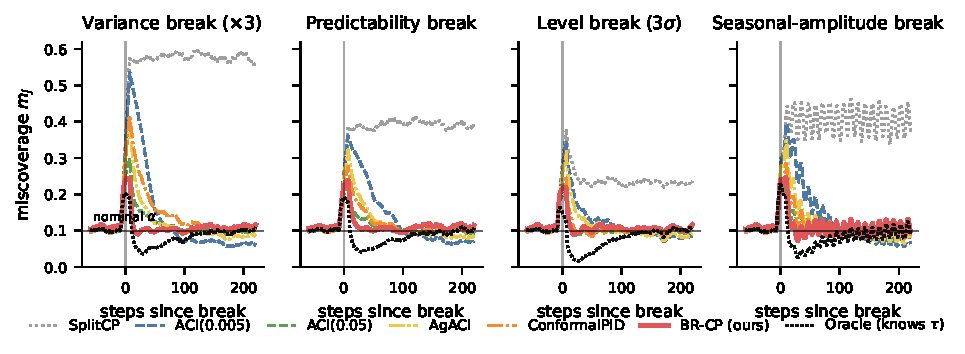
\includegraphics[width=\textwidth]{Fig1.pdf}
\caption{Instantaneous miscoverage $m_j$ around the break ($200$ seeds,
$15$-step moving average). All methods except split conformal attain marginal
coverage within $0.02$ of nominal, yet they differ by up to $27\times$ in the
area above the nominal line. \brcp{} (red) tracks the oracle (dotted black)
closely. The seasonal panel shows residual oscillation under the evaluated unconditioned-radius rules.}
\label{fig:debt}
\end{figure}

\begin{table*}[t]
\centering
\small
\caption{Coverage debt $\mathrm{CD}_\varepsilon$ at break magnitude $3$
($\varepsilon = 0.042$, $H=200$, $200$ seeds). Lower is better. The final
column is the mean over the seven break families; \textsc{none} is the
no-break control and quantifies the residual noise floor. The oracle is told
$\tau$; its \textsc{none} entry is an artifact of forcing a reset where there
is no break.}
\label{tab:cd}
\begin{tabular}{lrrrrrrrcr}
\toprule
Method & level & variance & trend & season & AR & predict. & drift &
\textsc{none} & \textbf{mean} \\
\midrule
Split CP & 20.67 & 87.15 & 134.69 & 53.55 & 23.09 & 50.13 & 3.58 & 0.02 & 53.27 \\
Rolling CP & 7.95 & 36.11 & 110.10 & 26.30 & 9.77 & 22.13 & 1.52 & 0.00 & 30.55 \\
ACI ($\gamma$=0.005)& 4.15 & 12.02 & 14.69 & 11.46 & 3.55 & 8.58 & 0.51 & 0.02 & 7.85 \\
ACI ($\gamma$=0.05) & 1.15 & 2.81 & 9.05 & 5.76 & 0.35 & 1.60 & 0.09 & 0.02 & 2.97 \\
EWA-ACI (local) & 3.10 & 4.93 & 6.95 & 7.60 & 1.66 & 4.20 & 0.59 & 0.02 & 4.15 \\
Conformal PI variant & 1.62 & 7.43 & 17.67 & 6.85 & 0.66 & 2.87 & 0.14 & 0.01 & 5.32 \\
\textbf{\brcp{} (ours)} & \textbf{1.41} & \textbf{1.85} & \textbf{2.72} &
 \textbf{5.58} & \textbf{0.41} & \textbf{1.62} & 0.42 & 0.13 & \textbf{2.00} \\
\midrule
\textit{Oracle (knows $\tau$)} & \textit{0.76} & \textit{1.22} & \textit{2.98} &
 \textit{3.06} & \textit{0.86} & \textit{1.04} & \textit{0.84} & \textit{0.78} &
 \textit{1.54} \\
\bottomrule
\end{tabular}
\end{table*}

\subsection{Marginal coverage masks post-break dynamics}

Table~\ref{tab:cd} and Figure~\ref{fig:debt} make the central point. Every
Several adaptive methods attain aggregate coverage near 0.90, but averaging across configurations can mask large deficits, especially under persistent trend breaks. For example, at trend magnitude 3, \brcp{} covers 0.8723 of evaluation points and ACI($0.05$) covers 0.8322, both far below nominal. At that configuration, their CD values are 2.72 and 9.05, respectively; the performance difference cannot be summarized solely by a nominal-coverage statement. Their coverage debts span $0.41$ to $134.69$.
Split conformal, which is what one gets by calibrating once on historical data,
under-covers by more than $30$ points for hundreds of steps and never recovers.

\subsection{Comparison with the oracle}

\brcp{} attains a mean debt of $2.00$ against $2.97$ for the best tuned fixed
step, $4.15$ for the EWA-ACI variant and $5.32$ for the PI variant, reducing the observed gap to the known-break-time reset policy ($1.54$) by $68\%$. It is numerically best among causal methods for variance, trend, and seasonal breaks at magnitude 3; faster ACI has lower CD in level, AR, predictability, and drift. Most of the seven-family mean benefit comes from trend: at magnitude 3, the trend CD reduction is $9.05-2.72=6.33$ of a total seven-family net reduction of approximately $6.80$ ($93\%$). Excluding trend, the reported rounded values give a mean of $1.96$ for ACI($0.05$) and $1.88$ for BR-CP, a much smaller difference. On marginal TTR-C it recovers in
$1$--$5$ steps on level, variance, AR, predictability and seasonal breaks,
against $1$--$25$ for ACI($0.05$) and $30$--$73$ for ACI($0.005$); the oracle
needs $0$--$2$.

The most practically relevant property is the scaling. As a variance break
grows from $2\times$ to $4\times$, \brcp{}'s debt moves only from $1.56$ to
$2.01$, because larger breaks are proportionally easier to detect and the
shorter delay offsets the higher per-step deficit. Over the same range
The evaluated PI variant degrades from $3.16$ to $11.98$ and ACI($0.005$) from $8.85$ to
$13.18$. This favorable variance-break pattern is limited to the tested magnitudes and should not be extrapolated to arbitrarily large shocks; the persistent trend family is a counterexample to a blanket robustness claim.

Paired Wilcoxon tests with Holm correction find \brcp{} significantly better on
early post-break miscoverage in $17$ of $21$ configurations against
ACI($0.005$), the EWA-ACI variant, rolling and split conformal, and $13$ of $21$ against
the PI variant. Against ACI($0.05$) the comparison is $9$ of $21$ in \brcp{}'s
favor with the reverse differences never exceeding $0.008$ in absolute value.
We want to be explicit about what this does and does not show. On transient
coverage \brcp{} and a well-tuned fast ACI are broadly comparable, and the
$2.00$ versus $2.97$ gap in mean debt is driven by the families where a fixed
fast step does badly (trend, season) rather than by a uniform advantage. What
separates the two is not the transient but the frontier: ACI($0.05$) and BR-CP trade lower debt against different observed volatility and width patterns
(Figure~\ref{fig:frontier}, right), and $\gamma=0.05$ was selected post hoc from the evaluated grid. Fair prospective comparisons require comparable development-data tuning for every method.

\subsection{Interval efficiency}

Post-break interval scores place \brcp{} within $3\%$ of every adaptive
baseline (Table~\ref{tab:winkler}), and its mean interval width is
\emph{narrower} than ACI($0.005$) and ACI($0.05$) on six of seven families, by
up to $4.6\%$. Because the widening is triggered rather than continuous, the
intervals are wide when the regime is unknown and tight otherwise, which is the
behavior the interval score rewards.

\begin{table}[t]
\centering
\small
\caption{Post-break interval (Winkler) score at magnitude $3$, in percent
relative to \brcp{}. Positive means worse than \brcp{}. Split conformal is
omitted from the mean; its penalty reaches $604\%$ on the trend break.}
\label{tab:winkler}
\begin{tabular}{lrrrr}
\toprule
Method & variance & predict. & level & season \\
\midrule
Rolling CP & $+9.3$ & $+2.9$ & $-1.2$ & $+3.1$ \\
ACI ($\gamma$=0.005) & $+2.3$ & $+0.0$ & $-1.6$ & $+0.3$ \\
ACI ($\gamma$=0.05) & $+2.4$ & $+1.1$ & $+0.8$ & $+0.8$ \\
EWA-ACI (local) & $+1.4$ & $-0.1$ & $-1.4$ & $+0.1$ \\
Conformal PI variant & $-1.1$ & $-2.2$ & $-1.0$ & $-1.1$ \\
\textbf{\brcp{}} & $0.0$ & $0.0$ & $0.0$ & $0.0$ \\
\bottomrule
\end{tabular}
\end{table}

\subsection{Fixed-step sensitivity}

\begin{figure}[t]
\centering
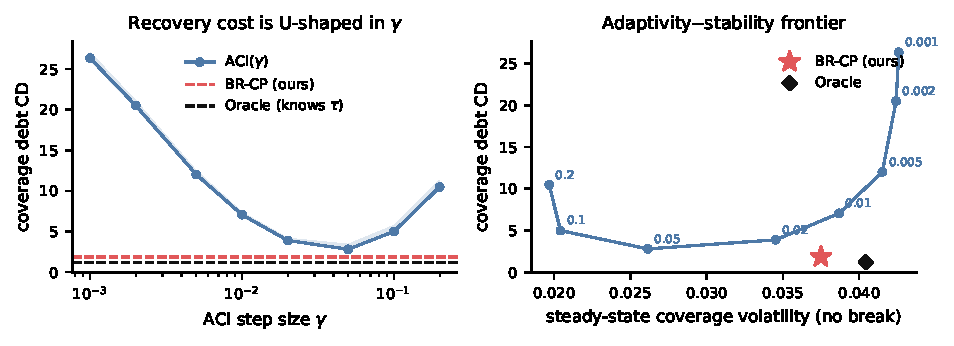
\includegraphics[width=0.92\textwidth]{Fig2.pdf}
\caption{Left: coverage debt of ACI as a function of $\gamma$ is U-shaped; the
best attainable value, $2.81$ at $\gamma=0.05$, still exceeds \brcp{}'s $1.85$.
Right: coverage-debt versus variability in empirical no-break coverage. BR-CP has lower CD than tested ACI steps, but not lower volatility at every operating point.}
\label{fig:frontier}
\end{figure}

Figure~\ref{fig:frontier} sweeps $\gamma$ over three orders of magnitude on the
variance break. Debt falls from $26.34$ at $\gamma=0.001$ to a minimum of
$2.81$ at $\gamma=0.05$ and then rises again to $10.47$ at $\gamma=0.2$, while
steady-state coverage on the no-break control degrades monotonically from
$0.9025$ to $0.8802$. \brcp{} attains $1.85$ at a steady-state coverage
volatility of $0.0375$, which on the ACI curve is larger than the volatility of ACI($\gamma=0.05$), even though BR-CP has lower CD. The plotted no-break coverage volatility is $0.0375$ for BR-CP and $0.0262$ for ACI($\gamma=0.05$), so BR-CP pays a measurable volatility cost; the figure does not establish dominance at both coordinates. Volatility here is the reported standard deviation of empirical coverage-rate estimates across no-break replications, not the step-to-step variation of interval radius or of $\alpha_t$.

\subsection{Detector-space comparison}

\begin{figure}[t]
\centering
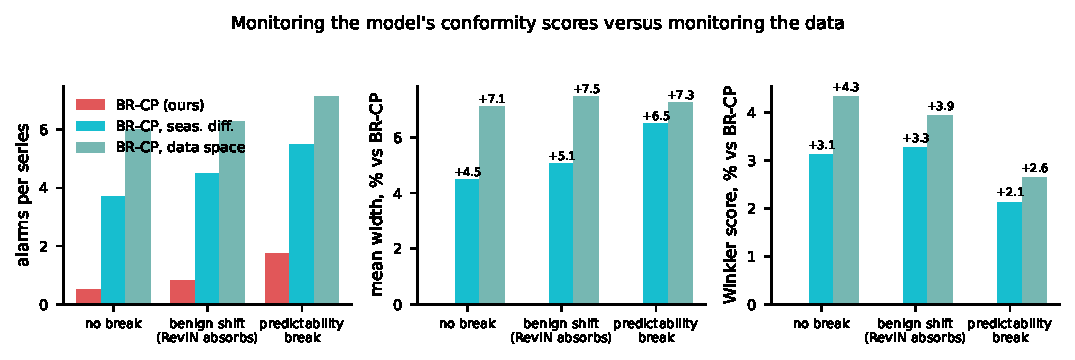
\includegraphics[width=0.92\textwidth]{Fig3.pdf}
\caption{Score-space versus data-space monitoring, identical CUSUM recursion.
At the tested, unmatched false-alarm operating points, monitoring observations produces more alarms and pays
$4.5$--$7.5\%$ in interval width and $2.1$--$4.3\%$ in interval score. On a
stationary seasonal series with \emph{no break at all} the data-space monitor
fires six times per series.}
\label{fig:detector}
\end{figure}

Figure~\ref{fig:detector} compares the identical detector applied to the score
stream, to the raw observations, and to seasonal differences, the strongest model-free way to strip predictable structure before monitoring in data space.
On a stationary series with no break, \brcp{} raises $0.52$ alarms per $800$
steps; the data-space variant raises $6.00$ and the seasonally differenced
variant $3.70$. Under a benign level shift absorbed by instance normalization
the counts are $0.82$, $6.27$ and $4.49$.

The consequence is not a coverage failure, since all three variants remain
valid and the trigger-happy ones are if anything slightly conservative, but a
systematic efficiency loss: $4.5$--$7.5\%$ wider intervals and $2.1$--$4.3\%$
worse interval scores across all three regimes. These findings compare the implemented operating points. They do not isolate the effect of monitored input because the false-alarm rates differ; a separately tuned, matched-ARL experiment is needed.
One might object that a better data-space monitor should first remove
predictable structure; the seasonal-difference variant does exactly that, and
narrows but does not close the gap. Taken to its conclusion, the objection is
the argument: removing predictable structure requires a model, and monitoring
the residuals of that model \emph{is} score-space monitoring.

\subsection{Ablation}

\begin{figure}[t]
\centering
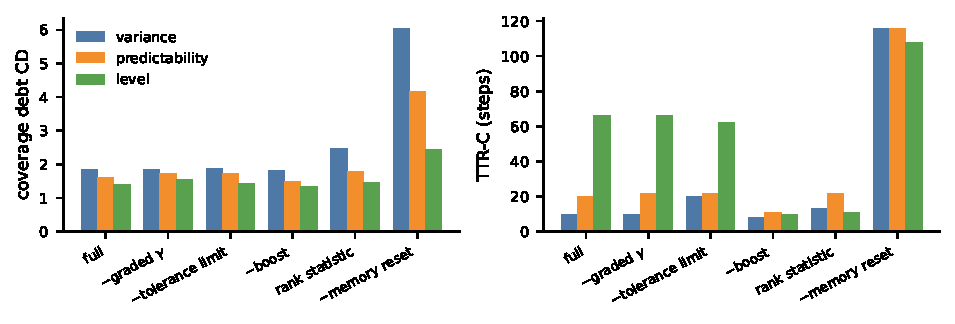
\includegraphics[width=0.92\textwidth]{Fig4.pdf}
\caption{Contribution of each mechanism. Removing the memory reset is
the most damaging; the rank-based detector statistic is uniformly slower than
the standardized one.}
\label{fig:ablation}
\end{figure}

In these tested ablations, removing the memory reset (R2) is especially costly: debt rises from $1.85$ to $6.05$ on
the variance break and from $1.62$ to $4.16$ on the predictability break, and
TTR-C from $10$ and $20$ steps to $116$. The graded step size (R1) contributes
a smaller but consistent gain ($1.55 \to 1.41$ on level, $1.73 \to 1.62$ on
predictability) at a small steady-state cost. Replacing the standardized
detector statistic by the rank-based statistic raises debt
to $2.46$ on the variance break and widens intervals by $2.0\%$, showing a longer delay for the tested rank-based operating point; a numerical rank cap alone cannot explain the result without accounting for threshold and slack normalization.

The 100-step post-alarm boost (an optional part of R1, not R4) is \emph{not} supported as an additional improvement: removing it leaves debt
statistically unchanged or marginally better ($1.81$ vs.\ $1.85$ on variance).
Once the graded step size and the reset are in place the boost is redundant, and
we report this rather than retaining a component the evidence does not justify.
A no-boost design may be preferable in deployment, but the main estimates in this paper still refer to the evaluated boosted implementation.

\subsection{Mechanism illustration}

\begin{figure}[t]
\centering
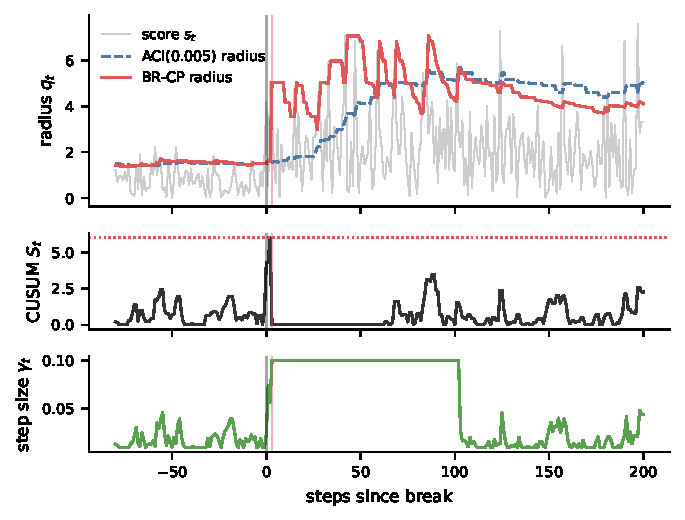
\includegraphics[width=0.86\columnwidth]{Fig5.pdf}
\caption{A single replication of the variance break. The CUSUM crosses its
threshold two steps after the break; the radius jumps immediately from $1.6$ to
$5$, where ACI($0.005$) needs about fifty steps to arrive. The radius is
visibly jumpy while the post-break buffer refills under the tolerance limit,
then settles.}
\label{fig:mechanism}
\end{figure}

Figure~\ref{fig:mechanism} traces one replication and makes concrete what the
aggregate numbers describe. The CUSUM statistic is near zero before the break,
so the step size sits at $\gamma_{\text{slow}}$ and the layer behaves like
conservative ACI. Two steps after the break the statistic crosses its
threshold; the memory reset discards the pre-break scores and the tolerance
limit, evaluated on the handful of post-break scores that triggered the alarm,
raises the radius from $1.6$ to about $5$ in a single step. ACI($0.005$) reaches
the same radius after roughly fifty steps. The visible jaggedness of the BR-CP
radius over the following hundred steps is the tolerance limit at work on a
buffer that is still small; as the buffer refills the margin contracts and the
radius settles onto a path slightly below ACI's, which is the width advantage
of Table~\ref{tab:winkler} seen at the level of a single series.

%======================================================================
\section{Controlled stress tests on real-world benchmarks}
\label{sec:real}

\subsection{Frozen cross-domain forecaster}

The simulation isolates the calibration layer, and that isolation is what makes
it insufficient on its own: real conformity scores are heavier tailed,
autocorrelated and heteroskedastic in ways synthetic AR noise is not. We
therefore repeat the core comparison using a frozen cross-domain linear
forecaster on real target series. This models the calibration aspect of
deployment, but is not an experiment with a published foundation model.

The archived protocol reports fitting a single global linear forecaster
once on $261$ training series drawn from \emph{electricity},
\emph{traffic} and \emph{weather} ($313{,}200$ context windows),
then freezing the resulting weights. This revision recovered the saved
weights and reproduced the target evaluation, but did not reproduce that
original pretraining from identical source files. It regresses the next value on an instance-normalized context window of $96$ observations and is frequency-agnostic. It is then applied, without retraining, to target
datasets reported as excluded from its fitted corpus: \emph{ETTh1},
\emph{ETTh2}, \emph{ETTm1}, \emph{ETTm2} and \emph{exchange rate}.
Because one recovered electricity file had the wrong benchmark schema,
we cannot independently certify exact training-data versions or
byte-level train/evaluation exclusion. The archived report describes
this as cross-domain transfer, and reports that mean absolute error is $0.31$--$0.51$ times that of seasonal naive on every held-out dataset. (\emph{Influenza} is
excluded: at $966$ weekly observations it cannot supply a calibration window, a
break window and a recovery horizon.)

Coverage debt is undefined without a known break time, and the natural regime
changes in these benchmarks are not dated. We therefore inject bounded,
non-cumulative breaks of identical size into the \emph{raw} target series, so
the frozen model forecasts the broken series exactly as it would in deployment
while $\tau$ is known exactly. Windows around every break, pooled across all
series, are the replications: $322$ break windows over $35$ series and
$368{,}081$ calibration steps per layer.

The full target-data arms (level, variance, no break) were replayed using the archived frozen forecaster and corrected deterministic Wilks cache. Across 35 series, the variance-arm BR-CP CD remained 3.210874 and coverage moved from 0.895914 to 0.895936; BR-CP-safe CD moved from 3.148036 to 3.144931, and its coverage moved from 0.896813 to 0.896819. These small changes do not eliminate the nominal-coverage deficit or establish fidelity to unimplemented published baselines.

\subsection{Detector recalibration}

The threshold selected on synthetic data, $(k,h)=(0.65,6.0)$, gives
$\mathrm{ARL}_0 = 1882$ there but only $642$ on real conformity scores. The
simulation's limitations section anticipated this; the size of the effect is
worth recording. Recalibrating on $75$ held-out series from the corpus
datasets, which are neither pretraining nor evaluation data, selects
$(k,h)=(0.8,8.0)$ with $\mathrm{ARL}_0 = 1744$. All real-data results below use
that operating point. Because real series contain genuine regime changes, this
is an upper bound on the false-alarm rate rather than a pure null, so the
threshold it implies is conservative.

\begin{table}[t]
\centering
\small
\caption{Controlled variance-shift stress test on five real-world benchmark datasets: $322$ break windows over $35$ held-out series. CD uses $\varepsilon=0.03344$ for $322$ pooled windows, whereas the synthetic arm uses $0.04243$ for $200$ seeds; TTR-C uses the 24-step marginal recovery criterion. The final column reports alarms per $1000$ steps on unbroken series.}
\label{tab:real}
\begin{tabular}{lrrrrr}
\toprule
Method & CD & TTR-C & cov. & Winkler & alarms \\
\midrule
Split CP & 114.05 & $\infty$ & 0.658 & 17.64 & 0.00 \\
Rolling CP & 43.02 & $\infty$ & 0.880 & 10.96 & 0.00 \\
ACI ($\gamma$=0.005) & 16.85 & 55 & 0.901 & 10.07 & 0.00 \\
ACI ($\gamma$=0.01) & 9.10 & 28 & 0.901 & 9.54 & 0.00 \\
ACI ($\gamma$=0.05) & 3.82 & 27 & 0.895 & 8.93 & 0.00 \\
ACI ($\gamma$=0.1) & 6.15 & 72 & 0.888 & 8.93 & 0.00 \\
EWA-ACI (local) & 4.67 & 43 & 0.893 & 8.92 & 0.00 \\
Conformal PI variant & 17.44 & $\infty$ & 0.899 & 9.74 & 0.00 \\
\textbf{\brcp{}} & \textbf{3.21} & \textbf{8} & 0.896 & \textbf{8.91} & 1.05 \\
\textbf{\brcp{}-safe}& \textbf{3.14} & \textbf{6} & 0.897 & 8.93 & 1.05 \\
\brcp{}, data space & 3.48 & 13 & 0.902 & 9.27 & 7.62 \\
\bottomrule
\end{tabular}
\end{table}

\begin{figure}[t]
\centering
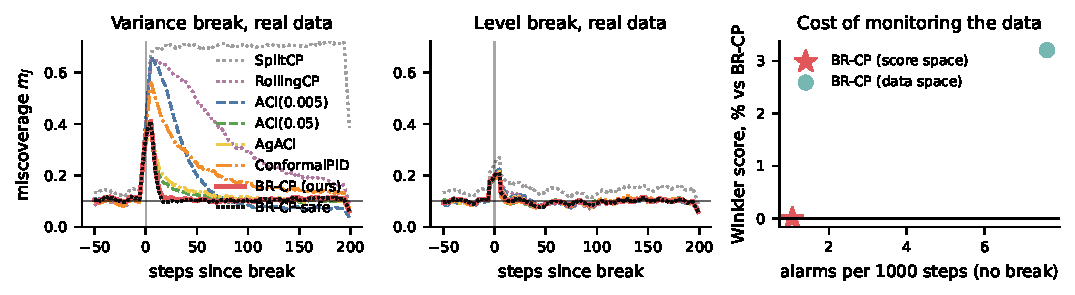
\includegraphics[width=0.92\textwidth]{Fig6.pdf}
\caption{Controlled stress tests on real-world benchmark series. Left: post-break miscoverage after a variance shift. Middle: a $3\sigma$ level shift has little effect after instance normalization. Right: on unbroken series, data-space monitoring produces substantially more alarms than score-space monitoring and a higher interval score.}
\label{fig:real}
\end{figure}

\subsection{Transfer results}

Table~\ref{tab:real} and Figure~\ref{fig:real} show the same method ranking for the variance-shift stress test. On the variance break \brcp{} attains the lowest coverage debt,
$3.21$ against $3.82$ for the best evaluated ACI, $4.67$ for the EWA-ACI variant and $17.44$ for
Conformal PID, and crosses the tolerance-adjusted 24-step moving-average recovery threshold in $8$ steps, versus $27$ to $55$ for selected adaptive baselines; the evaluated PI variant is censored beyond the reported horizon.
Early post-break miscoverage is $0.178$ against $0.205$ for ACI($0.05$) and
$0.387$ for the PI variant. Its Winkler interval score is $8.91$, compared with $8.93$ for ACI($0.05$) and $8.92$ for EWA-ACI.

Two further predictions transfer. First, monitoring the observations rather
than the conformity scores costs what the simulation said it would: on unbroken
real series the data-space variant raises $7.62$ alarms per $1000$ steps
against \brcp{}'s $1.05$, for $5.5\%$ wider intervals and a $3.2\%$ worse
interval score at the evaluated operating points, which are not matched for no-break false-alarm rate. Second, and more strikingly, the \emph{level} break is almost
benign on real data: every adaptive method scores a coverage debt near $1$ and
recovers within a step or two, consistent with attenuation of a level shift under the evaluated instance normalization. This controlled result, rather than the dated-event outcomes, supports the narrower interpretation that calibration should track model competence
rather than the data.

\subsection{Failure cases and attenuated effects}

We report three results that qualify the claim.

\textbf{The margin over a tuned fast ACI shrinks.} In simulation \brcp{} beat
ACI($0.05$) by $34\%$ on mean debt; here the gap is $16\%$ ($3.21$ vs $3.82$),
and a paired Wilcoxon test across the $35$ series finds \emph{no} significant
difference in interval score ($-0.14\%$, $p=0.49$), nor against the EWA-ACI variant
($-0.30\%$, $p=0.37$). The differences that are significant are against
ACI($0.005$) ($+12.2\%$, $p<10^{-4}$), ACI($0.01$) ($+6.4\%$), the PI variant
($+8.2\%$), rolling conformal ($+22.0\%$) and the data-space variant
($+3.2\%$). The defensible claim on real data is therefore that \brcp{}
has a small observed interval-score difference relative to the evaluated fast ACI and EWA-ACI variants; neither of the reported Wilcoxon comparisons detected a significant difference, while the tolerance-adjusted recovery estimates differed. Nonsignificance does not establish statistical equivalence.

\textbf{The safe reset slightly improves the perturbed-data point estimate.} \brcp{}'s marginal
coverage on real data is $0.896$; the safe-reset variant, which avoids increasing the internal miscoverage level on alarm (without guaranteeing a monotone radius), reaches $0.897$ with a slightly \emph{lower}
debt ($3.14$ in the corrected-cache replay; $3.15$ historically) and faster recovery ($6$ steps) at a $0.8\%$ width cost. A separate unbroken-series setting yields $0.900$. A newly calculated
35-series cluster bootstrap on the archived perturbed variance-test per-series
summary gives BR-CP coverage $0.895914$ (95\% percentile interval
$[0.894722,0.897162]$), safe coverage $0.896813$
($[0.895624,0.898049]$), and paired safe-minus-standard difference
$0.000899$ ($[0.000657,0.001144]$). These intervals resample whole series,
not individual prediction steps, and do not necessarily capture dependence
between series from the same benchmark. Neither result establishes that the method removes the nominal coverage deficit under injected breaks or in the simulations. The variant is a pragmatic alternative rather than a coverage-guaranteed default.

\textbf{Closely spaced breaks defeat the re-anchoring rule.} When a second
break of a different kind is injected $40$ steps after the first, inside the
$60$-step window during which the detector is disarmed and rebuilding its null,
\brcp{}'s debt rises to $4.28$, \emph{worse} than ACI($0.05$)'s $3.87$,
although recovery is still faster ($15$ versus $20$ steps). The safe variant
recovers part of it ($4.18$, $13$ steps). This is a real failure mode of
mechanism R4 and not a tuning artifact: while re-anchoring, the layer is blind.
Maintaining a shadow anchor from the pre-alarm regime could reduce this blind period and is left for future work.

\textbf{Threshold sensitivity.} Varying $h$ by $\pm30\%$ around the calibrated
value moves debt from $2.72$ ($h=5.6$, $38.1$ alarms per series, or $3.62$ per $1000$ steps) to $3.21$ ($h=8.0$, $27.3$ per series, or $2.60$ per $1000$ steps) to $3.48$ ($h=10.4$, $23.1$ per series, or $2.20$ per $1000$ steps), with marginal coverage
between $0.894$ and $0.897$ and mean width varying by under $1\%$. Across this sensitivity range, the main coverage and width conclusions remain similar. The most conservative threshold has higher debt than the calibrated setting, whereas the lower threshold trades more alarms for lower debt.



\subsection{Externally dated events}
\label{sec:cases}

The controlled real-data study injects breaks to obtain known break times and replicated
miscoverage curves. As a complementary descriptive analysis, we replayed two externally
dated events using the recovered \texttt{exchange\_rate.csv} and
\texttt{national\_illness.csv} inputs, the archived frozen global ridge forecaster,
and the same calibration implementations. The event dates are 15 September 2008
(Lehman Brothers bankruptcy) and 26 April 2009 (US H1N1 emergency
announcement). The first weekly influenza observation on or after the latter
date is 28 April 2009. These dates are external anchors, \emph{not} verified
statistical change points. There is one observed realization per series, so
we report realized miscoverage, rather than population conditional coverage
or a coverage-debt estimand.

The recovered run reproduces all \(84\) method-by-series rows from the
archived case-study CSV exactly, including full-period coverage, pre/post
miscoverage, width, and interval scores. The separate local trace export
contains \(32{,}480\) time-indexed records and allows us to correct a
bookkeeping error in the archived \texttt{alarm\_lag} column: the original
script subtracted the warm-up length a second time even though the alarm
index was already relative to the evaluation window. Table~\ref{tab:natural}
and Figure~\ref{fig:natural} report the corrected time origin and local
observed hit-rate trajectories. Method means in the table average equally
across the eight exchange-rate or four illness channels; they are not
independent replications of a break-probability distribution.

\begin{table}[t]
\centering\small
\caption{Observed pre/post miscoverage for the externally dated events.
The Lehman window contains \(260\) daily observations after the event, and
the H1N1 window contains \(60\) weekly observations. Post-event alarm counts
are from BR-CP's own CUSUM and are summed over channels; \emph{none} is
registered at offset zero. These are descriptive rates, not conditional
coverage estimates.}
\label{tab:natural}
\begin{tabular}{llrrrr}
\toprule
Event & Calibration method & Pre miscov. & Post miscov. & Channels & Post alarms\\
\midrule
Lehman & SplitCP & 0.0942 & 0.1808 & 8 & --\\
Lehman & ACI(0.05) & 0.1115 & 0.0971 & 8 & --\\
Lehman & BR-CP & 0.1000 & 0.0962 & 8 & 7\\
Lehman & BR-CP-safe & 0.0990 & 0.0947 & 8 & 7\\
H1N1 & SplitCP & 0.3083 & 0.2000 & 4 & --\\
H1N1 & ACI(0.05) & 0.1250 & 0.0917 & 4 & --\\
H1N1 & BR-CP & 0.1125 & 0.0917 & 4 & 0\\
H1N1 & BR-CP-safe & 0.1125 & 0.0833 & 4 & 0\\
\bottomrule
\end{tabular}
\end{table}

\begin{figure}[t]
\centering
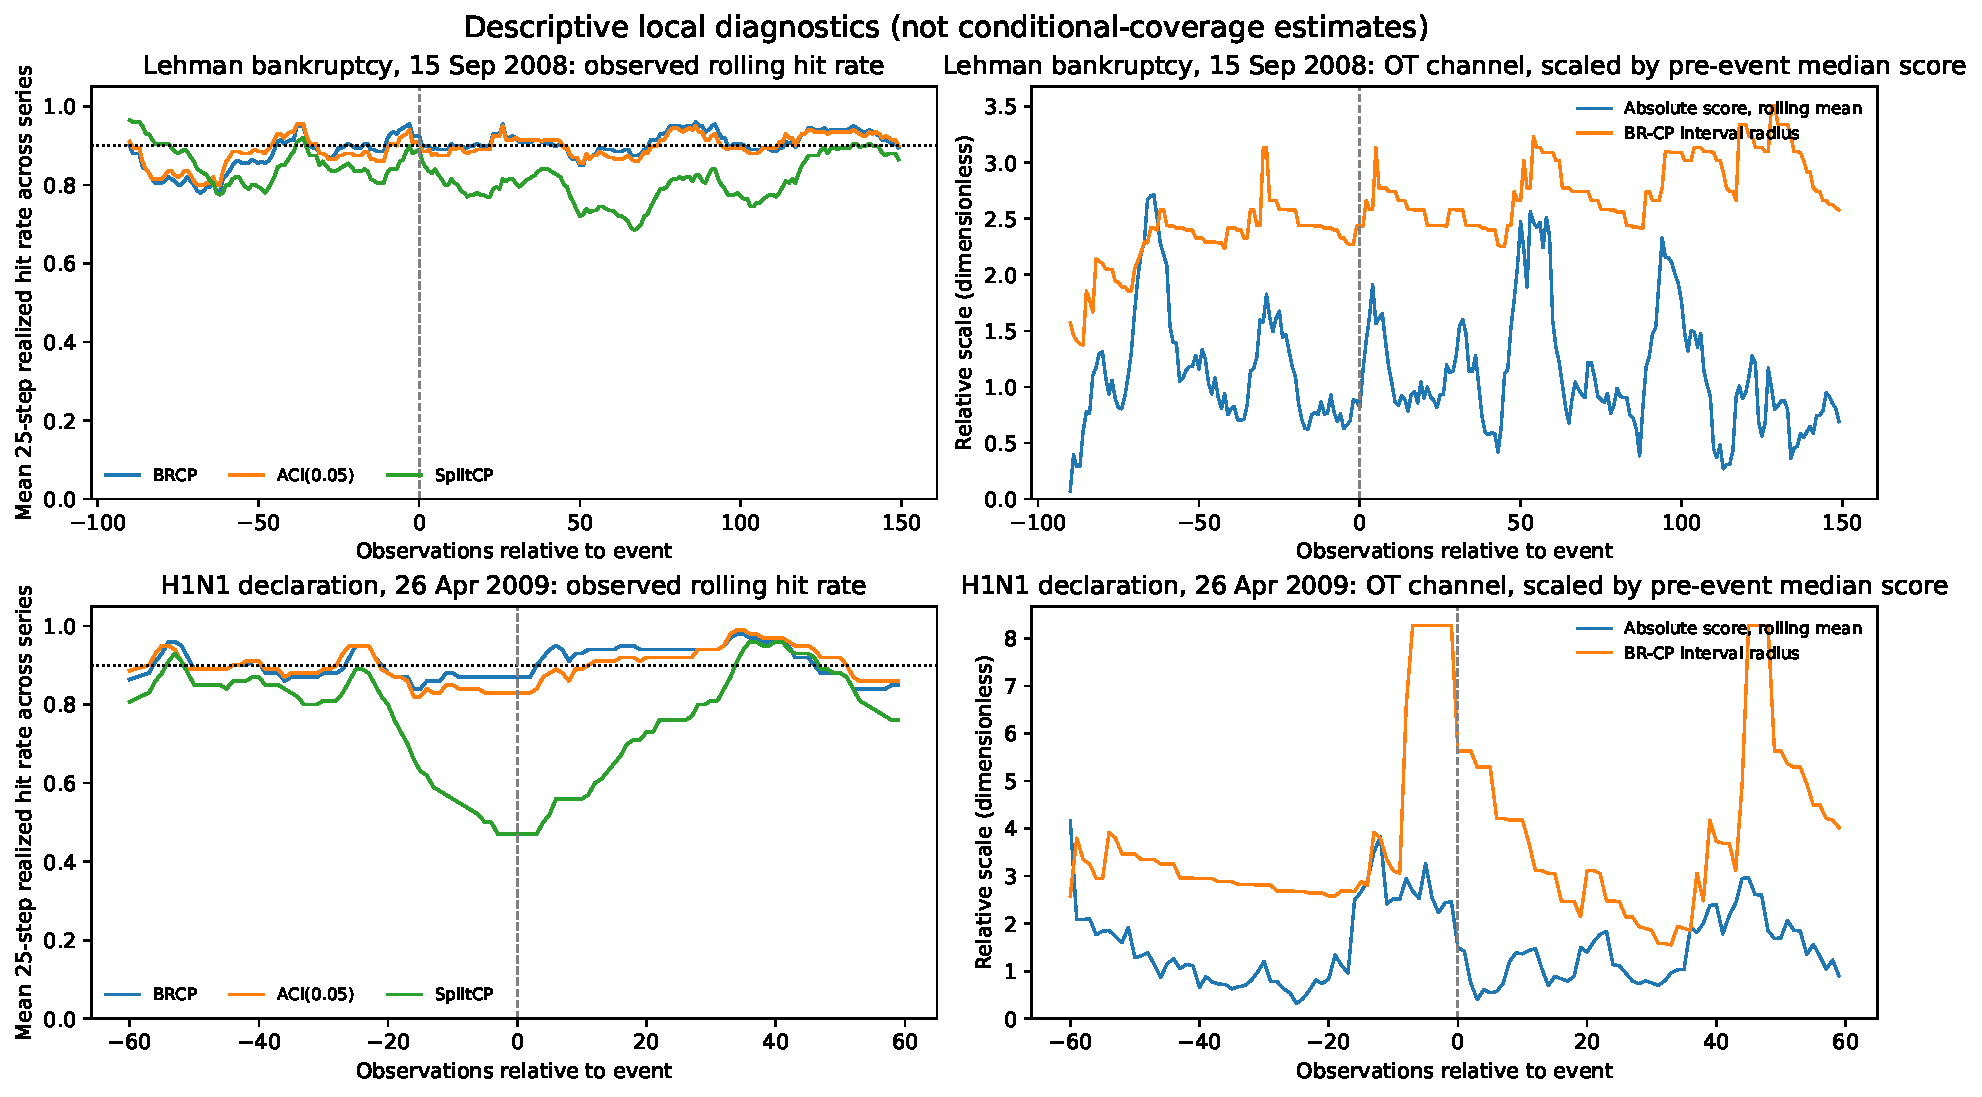
\includegraphics[width=\textwidth]{Fig7.pdf}
\caption{Replayed, descriptive local diagnostics around the two event dates.
Left panels show mean realized 25-step trailing hit rate over the respective
channels; right panels show the \texttt{OT} channel's absolute residual score
(rolling mean) and BR-CP radius, both normalized by its pre-event median
score. A vertical dashed line marks the prespecified external date. These
curves are not estimates of conditional coverage and do not validate a causal
event-induced break.}
\label{fig:natural}
\end{figure}

No BR-CP alarm occurs at offset zero for either event. During the \(260\)
post-Lehman daily observations, however, the score monitor raises seven
alarms over five of the eight channels. The earliest post-event alarm offsets
for those five channels are \(11,31,48,96,257\) observations; the remaining
three channels have no post-event alarm in the window. Thus the previous
statement that the detector produced \emph{no response} to Lehman was false:
it produced delayed and channel-specific responses, but no same-day alarm.
During the \(60\)-week post-H1N1 window, it raises no alarms in the four
illness channels. Alarm-free windows do not imply the absence of local score
variability: the empirical 25-step hit rates vary visibly near both event
dates. For Lehman, the mean observed BR-CP miscoverage changes from 0.1000
to 0.0962 across the pre/post windows, whereas static split conformal changes
from 0.0942 to 0.1808. For H1N1, BR-CP changes from 0.1125 to 0.0917;
neither pooled average establishes a population-level conditional statement.

The source CSVs have the expected columns and date ranges and have been
hashed in the accompanying replication audit. Their exact byte identity to
the upstream public release remains unverified. The replacement
\texttt{electricity.csv} found elsewhere on the connected Drive is \emph{not}
the THUML Electricity benchmark and is excluded from any claim of newly
retrained pretraining; the event study instead uses the previously archived
frozen forecaster, unchanged. These considerations limit external validity,
and no causal claim is made for the effectiveness or failure of detection at
the external event dates.


\paragraph{Real variance-arm mechanism audit.}
The new full 35-series variance-arm replay was independently instrumented
for the published implementations ACI($0.05$) and BR-CP. Both outputs
match the deterministic corrected-cache full replay in all coverage, width,
interval-score, and total-alarm fields for the $35$ paired series. Across
$368{,}081$ evaluated forecasts per method, ACI($0.05$) projects its
internal level at $4{,}463$ updates ($1.213\%$), evaluates a nonpositive
level at $4{,}315$ radii, and caps $803$ further finite empirical quantiles
at the sample maximum. For BR-CP, the corresponding update projections
number $1{,}720$ ($0.467\%$); nonpositive-level radii number $952$, and
there are $66$ finite empirical-quantile caps. The BR-CP implementation
enters the Wilks-inspired small-buffer order-statistic calculation
$210{,}648$ times and uses the empirical maximum because no order statistic
meets the nominal fixed-i.i.d. criterion on $6{,}247$ occasions ($2.966\%$).
Neither of these two methods emits an infinite radius in this replay.
These are implementation frequencies, not validity guarantees, and should
not be extrapolated to published AgACI/PID or other stress-test arms.
The per-series count CSV and an instrumented script are included in the
revision audit as separately versioned evidence.

\subsection{Remaining validation}

Our forecaster is a small global model, not a published checkpoint. The
protocol above is checkpoint-agnostic: \texttt{scripts/run\_tsfm\_real.py}
implements the same interface for Chronos-Bolt and TimesFM.
The detector threshold is likely to require re-estimation because the conformity-score dependence structure changes with the forecaster and dataset. Confirmatory evaluation on published checkpoints and multi-horizon calibration remain future work.

\section{Additional uncertainty and mechanism checks}
\label{sec:extra}

\paragraph{Tolerance sensitivity.}
We recomputed CD directly from archived per-replication error curves,
without running new forecasts. Table~\ref{tab:eps} averages the $21$
synthetic break cells, and includes $\varepsilon=0$. The method ranking
shown here persists over the examined grid, but this is an empirical
observation, not a mathematical invariance of rankings.
\begin{table}[t]
\centering\small
\caption{Mean synthetic CD over 7 families, 3 magnitudes, 200 paired seeds per
cell. Results recalculated from released per-offset error arrays.}
\label{tab:eps}
\begin{tabular}{lrrrr}
\toprule
$\varepsilon$ & BR-CP & ACI(0.05) & EWA-ACI (local) & PI variant \\
\midrule
0.000 & 5.450 & 6.351 & 7.986 & 9.311 \\
0.020 & 3.230 & 4.285 & 5.686 & 7.046 \\
0.04243 & 1.915 & 2.828 & 4.001 & 5.356 \\
0.050 & 1.651 & 2.468 & 3.591 & 4.903 \\
0.070 & 1.203 & 1.712 & 2.748 & 3.870 \\
\bottomrule
\end{tabular}
\end{table}

\paragraph{Real-data dependence and weighting.}
The $322$ stress-test windows are nested within $35$ held-out series. In
Table~\ref{tab:real}, every window receives equal weight; thus series
contribute in proportion to their number of windows. To assess sensitivity,
we resampled \emph{entire series} with replacement ($2{,}500$ draws),
retaining all windows within each resampled series and recomputing the
nonlinear CD estimator. The paired bootstrap distribution for
$\mathrm{CD}_{\rm ACI(0.05)}-\mathrm{CD}_{\rm BRCP}$ has a percentile
range of $[0.261,1.017]$ with observed difference $0.611$. The same
35-series resampling yields marginal TTR-C of 8 steps (percentile range
$[7,9]$) for BR-CP and 27 ($[25,32]$) for ACI($0.05$).
These are uncertainty intervals for the operational period-average recovery
estimator, not intervals for an unobserved population individual-series
recovery time.
Equal weighting of the $35$ series instead yields BR-CP CD $3.251$
and ACI(0.05) CD $3.788$, compared with window-weighted CD $3.211$
and $3.822$. This cluster procedure accounts for within-series windows,
but not necessarily dependence across series from the same benchmark.
Since CD applies a positive part to estimated probabilities, bootstrap
intervals for individual method CD can be shifted upward; paired
\emph{differences} are emphasized rather than declaring strict coverage
of the observed plug-in point estimate by marginal intervals.

On the real variance-stress-test curves, $\varepsilon=0$ gives CD $5.532$
for BR-CP versus $6.780$ for ACI(0.05); the reported main-data tolerance
$0.03344$ gives $3.211$ versus $3.822$, while $0.042$ gives $3.043$ versus
$3.463$. The tolerance-adjusted 24-step marginal TTR-C is $8$ versus $27$
at the main tolerance and $64$ versus $130$ at $\varepsilon=0$.
Recovery estimates beyond the horizon are censored, not assigned a true
recovery time of $201$.

\paragraph{Detector-plus-reset-only ablation.}
We added an explicit implementation-level ablation consisting of the same
score-CUSUM, its detected reset-location rule, and fixed-step clipped ACI
($\gamma=0.01$), but \emph{without} graded adaptation, the 100-step fast
phase, or the small-buffer tolerance adjustment. This is an internal
\emph{detector-plus-reset-only} reference and is not presented as a
reproduction of any published CUSUM-reset method. Across the $21$ synthetic
break cells, mean CD was $2.406$ for this baseline versus $1.915$ for the
main BR-CP. The improvement is heterogeneous: at magnitude 3, trend CD
was $6.981$ versus $2.716$, but seasonal CD was $4.998$ versus $5.581$,
and slow-drift CD was $0.206$ versus $0.425$. These comparisons help
isolate when the additional mechanisms help and when they cost debt.


\subsection{Boundary conventions, detector-matching attempt, and reset-buffer audit}
\label{sec:checks}

\paragraph{ACI boundary sensitivity (new independent synthetic replay).}
The practical implementations in the main tables project the internal ACI
miscoverage level onto $[0,1]$ and cap unresolved upper quantiles at the finite
buffer maximum. To quantify the effect of this choice, we independently
replayed $60$ newly generated seeds per condition (seeds 40000--40059), using
the same frozen-forecaster generator, under a second convention: the
\emph{unprojected} ACI recursion, for which empirical quantiles outside the
unit probability range yield infinite or empty sets. The latter convention
preserves the unprojected coverage-control logic but sometimes makes interval
width and Winkler score infinite or undefined. These are new, separately
seeded checks and do not replace the original simulation grid.
\begin{table}[t]
\centering\small
\caption{New synthetic ACI boundary-convention audit, 60 independent seeds per
row and 48,000 evaluated steps per row. ``$+\infty$'' counts emitted infinite
radii; efficiency comparisons for that convention are not finite.}
\label{tab:aci-boundary}
\begin{tabular}{llrrrr}
\toprule
Break & $\gamma$ & clipped cov. & unprojected cov. & clipped projections & $+\infty$ radii \\
\midrule
No break & 0.05 & 0.8995 & 0.8998 & 89 & 397 \\
No break & 0.20 & 0.8810 & 0.8998 & 2,690 & 10,323 \\
Variance & 0.05 & 0.8941 & 0.9000 & 705 & 2,473 \\
Variance & 0.20 & 0.8626 & 0.8998 & 4,182 & 14,409 \\
Trend & 0.05 & 0.8320 & 0.8975 & 6,236 & 18,743 \\
Trend & 0.20 & 0.7336 & 0.8987 & 11,947 & 29,413 \\
\bottomrule
\end{tabular}
\end{table}
For example, at trend magnitude 3 with $\gamma=0.05$, using the unprojected
boundary raises whole-period coverage from 0.8320 to 0.8975, but $39.0\%$
of emitted intervals have infinite radius. The original ACI rule cannot
therefore be compared with the capped finite-radius implementation on mean
finite width without explicitly reporting this cost. The new audit script and
per-seed results are included in Online Resource 1.

\paragraph{Development-targeted false-alarm matching (new synthetic
replication).}
To improve comparability across detector spaces, we separately selected the
threshold for score-space and raw-data-space Page-CUSUM on $50$ independent
no-break development streams (seeds 10000--10049). We held
$k=0.65$, the standardized statistic, the $250$-point anchor and $60$-score
re-arm rule fixed. On a fixed threshold grid, the targets were 0.5 alarms
per 800 no-break evaluation steps; the selected thresholds were $h=5.75$
(score) and $h=10.50$ (data), producing 0.46 and 0.50 alarms per 800
\emph{development} steps. These settings were not reselected on test data.
\begin{table}[t]
\centering\small
\caption{Held-out synthetic detector-space replay (60 paired test seeds,
30000--30059). CD uses 200 offsets and $\varepsilon=0.04243$. Development
false-alarm targets were similar, but the held-out null rates diverged; this
is not a perfectly matched-ARL experiment.}
\label{tab:detector-matched}
\begin{tabular}{lrrrrrr}
\toprule
 & \multicolumn{2}{c}{No-break alarms/800} & \multicolumn{2}{c}{Variance CD} & \multicolumn{2}{c}{Predictability CD} \\
Detector & development & test & test & test TTR-C & test & test TTR-C \\
\midrule
Score, $h=5.75$ & 0.46 & 0.517 & 2.517 & 4 & 2.444 & 8 \\
Data, $h=10.50$ & 0.50 & 0.833 & 3.564 & 10 & 2.085 & 16 \\
\bottomrule
\end{tabular}
\end{table}
In the independent test null series, score and data monitors raised 0.517
and 0.833 alarms per 800 steps, respectively; a paired seed bootstrap gives a
95\% percentile interval of approximately $[0.00,0.65]$ for the
\emph{data-minus-score} alarm-count difference. The difference in operating
points persists despite calibration on development data. The data monitor also
had lower CD in the predictability setting but slower event detection
conditional on alarm, so the results do not establish universal superiority of
score-space monitoring. We retain the previously reported comparisons as
\emph{unmatched} and do not draw an isolated causal monitoring-space conclusion
from either study. More development samples, direct ARL$_0$ matching and
additional held-out real series are needed.

\paragraph{R3 fallback and ACI projection counts (new synthetic subset).}
We instrumented all BR-CP radius evaluations in the $60$ held-out test seeds
across the no-break, level, variance, season and predictability arms, with the
\emph{new matched-development score threshold $h=5.75$}, not the main-table
$h=6.0$ setting. Across 240,000 emitted score-space intervals, there were
347 projected-level updates and 233 finite-maximum quantile caps (including
226 evaluations at $\alpha_t\le0$). The R3 small-buffer order statistic was
called 98,022 times; on 3,240 of these calls ($3.31\%$), no order statistic
met the nominal 90\% Wilks confidence criterion and the code used the
sample maximum. These event counts are direct code instrumentation under the
specified exploratory-threshold protocol; they are not extrapolated to the
original 21-cell main simulation or to the real-data arm. The maximum fallback
is \emph{not} certified at 90\% confidence for its selected, dependent buffer.


\paragraph{Full 21-cell historical-configuration replay (new confirmed synthetic audit).}
We additionally instrumented all seven break families at all three magnitudes,
using the original seeds $0$--$199$ and the original main operating point
$k=0.65,h=6.0$. Crucially, this historical-configuration replay used the
same ordered BR-CP-then-OracleCP evaluation as the released program: the
original tolerance-order-statistic cache was process-global, so running the
methods in a different order can change later quantiles. The replay
reproduced the archived \emph{per-seed} BR-CP coverage exactly and width to a
maximum absolute numerical discrepancy of $7\times10^{-12}$.
Across $3{,}360{,}000$ emitted BR-CP intervals, the R3 rule was invoked
$1{,}678{,}992$ times; $147{,}341$ calls ($8.78\%$) fell back to the sample
maximum. The BR-CP adaptive level was projected back onto $[0,1]$ after
$23{,}810$ updates ($0.709\%$ of steps); $20{,}509$ subsequent radius
evaluations occurred at $\alpha_t\le0$, and $211$ other unresolved finite
quantile levels were capped at the sample maximum. No infinite-radius
intervals were emitted. The fallback is not an i.i.d. tolerance certificate.
\begin{table}[t]
\centering\small
\caption{New instrumentation for the complete historical synthetic main grid
(200 replications at each of three magnitudes per family; $h=6.0$).
The final column counts projected BR-CP calibration updates, not ACI updates.}
\label{tab:full-wilks}
\begin{tabular}{lrrr}
\toprule
Family & R3 calls & Max fallback & Projected updates \\
\midrule
AR & 298,044 & 18,140 & 2,469 \\
Level & 191,471 & 4,073 & 463 \\
Predictability & 233,625 & 7,336 & 856 \\
Season & 199,639 & 6,782 & 792 \\
Slow drift & 196,250 & 4,333 & 510 \\
Trend & 336,835 & 98,031 & 17,777 \\
Variance & 223,128 & 8,646 & 943 \\
\midrule
Total & 1,678,992 & 147,341 & 23,810 \\
\bottomrule
\end{tabular}
\end{table}

\paragraph{Full original clipped-ACI baseline audit.}
For the two fixed-step ACI baselines, we separately replayed the complete
$21\times200$ original synthetic configurations and checked every seed against
the archived coverage and width outputs (agreement at numerical precision).
For ACI($0.005$), $4{,}484/3{,}360{,}000$ updates ($0.133\%$) were projected
onto $[0,1]$; $4{,}647$ radii were evaluated at $\alpha_t\le0$ and $38{,}337$
additional finite-quantile evaluations were capped at the sample maximum.
For ACI($0.05$), the corresponding counts were $88{,}828/3{,}360{,}000$
($2.644\%$), $88{,}719$, and $8{,}207$. Neither clipped/capped ACI
implementation emitted infinite radii. These quantities concern the main
\emph{modified} ACI baselines, not the separate unprojected ACI sensitivity
study in Table~\ref{tab:aci-boundary}.

\paragraph{Deterministic cache correction and sensitivity.}
The archived implementation keyed the Wilks-order-statistic memoization on
$\alpha_t$ rounded to three decimal places, but calculated the initial cached
answer using the unrounded level. Consequently, different ordering of
BR-CP and OracleCP could produce different later interval radii. We corrected
the numerical cache in a separately versioned source fork: the lookup key
and order-statistic calculation now use the same level rounded to twelve
decimal places. An independent full 21-cell, 200-seed replay with this fix
changed cell-average BR-CP coverage by at most $3.75\times10^{-5}$ and
cell-average mean width by at most $0.00104$ in absolute value. BR-CP mean
CD over the 21 break cells changed from $1.91538$ to $1.91467$; the
magnitude-3 mean changes from $2.00117$ to $2.00154$, leaving the
conclusions at the reported two-decimal precision unchanged. The original
archive, corrected implementation, per-seed comparisons, and provenance
are supplied separately so the numerical correction is not hidden.


%======================================================================
\section{Post-hoc published-checkpoint robustness audit}
\label{sec:chronos_posthoc}

We additionally performed a \emph{post-hoc, exploratory} one-step experiment
with the frozen public Chronos-Bolt Small checkpoint
(revision \texttt{772f3d25d38aec6d914c8949dab4462e2d46f5d8}). This is
\emph{not} the source of the historical numerical claims in
Sections~\ref{sec:design}--\ref{sec:real}, and it does not establish
training-corpus disjointness or strict zero-shot evaluation. It uses
six public evaluation datasets (ETTh1, ETTh2, ETTm1, ETTm2, exchange
rate, illness), six evaluated channels per dataset (36 in total),
three scenarios per channel (unperturbed, level pulse, variance pulse),
and nine locally implemented calibration methods (108 scenario streams,
972 method--stream records). The original Chronos study classifies ETT
(hourly and 15-minute variants) and Exchange Rate among the 27
\emph{zero-shot evaluation} benchmark families excluded from its
training sets (Ansari et al., 2024, Table~3). The Chronos-Bolt model
card describes zero-shot testing on the corresponding benchmark suite.
These family-level documents support benchmark-intent separation for
five of the six named datasets; they do not verify byte-level identity
of our THUML files with those benchmark versions, and they do not
certify the training membership of national illness. We therefore
report these as public benchmark-provenance evidence, not a verified
six-file pretraining-disjointness guarantee. Detector thresholds in this
post-hoc arm were selected using one held-out channel per dataset, with
remaining channels reserved for evaluation. These channels are disjoint
but not statistically independent: they share dataset-level temporal
structure, so the test is not a new-domain, independent hold-out. Each
method uses the \emph{same cached}
Chronos median forecasts for its corresponding stream, enabling a
paired comparison. A level or variance intervention lasts 120 time steps
and then returns to baseline; this engineered return is a second change.

\paragraph{Corrections before analysis.}
Our first GPU notebook had two defects. It passed the conformal rank
$k=\lceil(n+1)(1-\alpha)\rceil$ as probability $k/n$ into a
``higher'' interpolation quantile, selecting the next order statistic
when $k<n$. We replaced this with the direct one-based rank $k$,
retaining the documented finite sample-maximum fallback when $k>n$;
the latter does not prove finite-sample validity under adaptive,
dependent scores. We replayed all 972 records from the original
saved forecast traces without running inference again, and added
114 order-statistic tests. The original detector search over
$h\leq20$ was also too narrow to match data-space and score-space
alarm frequencies. A \emph{post-hoc expanded development grid}
selected $h_{\rm score}=10$ and $h_{\rm data}=500$; on unperturbed
evaluation streams the observed rates were respectively $0.4861$ and
$0.5637$ alarms per 800 steps (difference $0.0777$ against the
numerical tolerance $0.15$). This is matching of \emph{empirical}
alarm counts, not an independently confirmed equality of null false-alarm
rates. The grid was expanded after the previous test mismatch became
known, so this analysis is not held-out confirmation.

\paragraph{Recovery estimates without the return break.}
Because the injected pulse ends at offset 120, computing coverage debt
over 150 offsets would confound the original intervention with the
engineered return. We therefore report \emph{exploratory} $\mathrm{CD}_{\varepsilon,100}$
and TTR-C on offsets $j=0,\ldots,99$, each before the return. At each
offset, we average the binary errors across repeated injected events
\emph{within} a channel and then average across the 36 channels.
For the 24-step rolling-average first-crossing TTR-C, the earliest
$j\leq76$ satisfying $24^{-1}\sum_{r=j}^{j+23}\widehat m_r
\leq\alpha+\varepsilon$ is reported; if none exists, TTR-C is
right-censored. A separate strict measure requires 25 consecutive
\emph{marginal-offset} values below the threshold and is censored
unless such a sequence occurs by offset 75. Neither statistic is a
conditional-coverage guarantee, and first crossing need not be persistent.
We illustrate $\varepsilon=0.03344$, which is a sensitivity point
reused from the historical real-data analysis, \emph{not} a newly
validated confidence bound for these 36 related channels.

\begin{table}[ht]
\centering
\small
\caption{Exploratory post-correction Chronos-Bolt Small audit.
CD100 and TTR24 are computed before the offset-120 return break,
with $\alpha=0.10$, $\varepsilon=0.03344$. TTR24 is the first
24-step rolling-average crossing; strict25 is a different condition.
``$>75$'' denotes right censoring of strict25 in the 100-step window.}
\label{tab:chronos_posthoc}
\begin{tabular}{llrrrr}
\toprule
Pulse & Wrapper & Coverage debt 100 & TTR24 & Strict25 & Mean miscoverage \\
\midrule
Level & ACI($0.05$) & 1.398 & 1 & 17 & 0.107 \\
Level & \brcp{} & 1.709 & 1 & 17 & 0.109 \\
Variance & ACI($0.05$) & 4.217 & 30 & $>75$ & 0.161 \\
Variance & \brcp{} & 3.431 & 6 & $>75$ & 0.138 \\
\bottomrule
\end{tabular}
\end{table}

In the exploratory variance pulse, \brcp{} has lower CD100 and earlier
rolling-average first crossing than ACI($0.05$), but both strict25
recovery estimates are censored in the observed 100-step window.
Under a level pulse, ACI($0.05$) has the lower CD100, and both
rolling-average TTR values equal one. These rankings depend on the
estimand: with $\varepsilon=0$, the CD100 values are respectively
$4.581$ versus $6.267$ for variance and $2.660$ versus $2.210$ for
level (\brcp{} versus ACI). A paired percentile bootstrap that
resamples the \emph{six datasets} as blocks (retaining their channels,
repeated interventions, and method pairing) gives exploratory
95\% intervals for CD100 differences (\brcp{} minus ACI) of
$[-1.134,-0.518]$ under variance and $[0.108,0.744]$ under level
at $\varepsilon=0.03344$. Six dependent domain blocks are too few
for strong inferential guarantees, and these intervals describe this
post-hoc estimator rather than a registered confirmatory effect.

On variance-pulse channels, the \emph{within-channel} BR-CP/ACI
Winkler score ratio is below one for only 8 of 36 channels,
with a median ratio $1.0146$ (higher means worse for BR-CP).
Raw mean Winkler scores are not scale-comparable across the illness,
exchange and ETT datasets. Thus the supplementary experiment does
\emph{not} establish across-the-board efficiency superiority, and
neither the simplified PI baseline nor the evaluated EWA-ACI variant
should be misrepresented as exact reference implementations.

The full original GPU result, corrected portable CPU replay,
per-event error traces, hash manifest, numerical tests, detector
grid, epsilon sensitivity, and dataset-block bootstrap are archived
as \emph{separately versioned} exploratory evidence. A newly chosen
hold-out, independent training-corpus audit, and full published
baseline fidelity remain outstanding. No results from this exploratory
checkpoint arm are mixed with the historical cross-domain forecaster's
main tables.


%====================== Independently seeded audit ========================
\section{Independent-seed detector null diagnostic and source fidelity}
\label{sec:fresh_detectors}

\paragraph{Pre-frozen diagnostic design (separate from Chronos).}
To probe whether our detector-space comparison remains fair on genuinely
new data, we created a separate \emph{detector-only} synthetic audit with
independent seeds, a correctly specified stationary Gaussian AR(1) null
($\phi=0.6$), and persistent level and innovation-variance changes.
Each series has 1,100 observations, with a 300-step detector warm-up,
250-point initial anchor, 60-point post-alarm re-anchoring, two-sided
standardized/winsorized Page increments ($k=0.8$), and 800 monitored steps.
The level intervention adds $(1-\phi)\,2$ to innovations starting at
$t=650$, while the variance intervention triples innovation scale;
when these interventions are absent, the data-generating law is exactly
stationary. Residual scores use the frozen, correctly specified AR(1)
one-step predictor. A fixed grid was selected using 90 independent
\emph{development} seeds to target 0.5 alarms per 800 null steps.
The selected thresholds ($h_{\mathrm{score}}=5$, $h_{\mathrm{data}}=16$)
were then evaluated \emph{once} on 300 disjoint test seeds, without
retuning. This is not a Chronos or BR-CP interval-coverage experiment.

\begin{table}[ht]
\centering
\small
\caption{New, independent-seed AR(1) detector-only diagnostic. The
prespecified alarm-rate difference tolerance is 0.20 alarms per 800
steps; observed test difference 0.3533 \emph{fails} that matching gate.
Post-shift hit rate is at least one alarm in the first 120 steps. These
hit rates are descriptive, \emph{not} a false-alarm-matched power comparison.}
\label{tab:fresh_detectors}
\begin{tabular}{lrrr}
\toprule
Detector & Null alarms / 800 & Level hit rate & Variance hit rate \\
\midrule
Score-space ($h=5$) & 0.5300 & 0.7067 & 0.9800 \\
Data-space ($h=16$) & 0.1767 & 0.9833 & 0.9733 \\
\bottomrule
\end{tabular}
\end{table}

The test null alarm-rate gap (score minus data) was $0.3533$ per
800 steps; a paired seed bootstrap (5,000 draws) gave an exploratory
95\% percentile interval $[0.250,0.453]$. Thus even with
independent development selection, a true no-change process and
fresh test seeds, the empirical matching target did \emph{not}
transport to the hold-out. We did not reselect thresholds using test
results. Accordingly, the post-change hit-rate comparison cannot
isolate monitoring-space effects at equal false-positive operation.
The variance-pulse conditional median delay among detected streams
was 3 steps for score-space and 24 for data-space, whereas under a
level shift score-space had the lower observed hit probability; these
are ancillary descriptive quantities under \emph{unequal} test alarm
budgets. This test does not prove any universally superior detector.
The frozen protocol, raw per-seed outcomes, explicit code and a
150-case equivalence test against the original Python detector are
included with the supplementary audit.


\paragraph{Sequential calibration-stability follow-up (exploratory).}
The previous 90-development-seed experiment failed to transfer its
false-alarm budget to the first test sample. We therefore ran a
\emph{sequential exploratory follow-up}, specifying its new seeds and
threshold grid before inspecting each new outcome but \emph{after}
observing the first failure. A larger calibration sample (1,200
new development seeds) selected $h_{\rm score}=5$ and
$h_{\rm data}=13$; on 900 disjoint new stationary-AR(1) null seeds
these yielded $0.5344$ and $0.4822$ alarms per 800 steps, a difference
of $0.0522$ (paired-bootstrap 95\% interval $[-0.018,0.122]$), within
that follow-up's stated tolerance of $0.15$. Without any further
threshold adjustment, a third independent set of 1,000 null seeds
yielded $0.524$ and $0.492$ alarms per 800 steps (gap $0.032$;
bootstrap difference interval $[-0.027,0.093]$). Thus larger
\emph{development} samples improved calibration stability for this
particular exactly stationary synthetic null. These follow-up choices
were motivated by inspecting the earlier result and are \emph{not}
an a priori registration of the entire sequence of studies.

On the third set of independently seeded persistent shifts, the
120-step detection proportions were $0.984$ (score) versus $0.977$
(data) for innovation-variance changes, with a paired hit-rate
difference of $0.007$ (bootstrap interval $[-0.005,0.019]$);
the conditional median detection delays were 3 versus 17 steps.
For persistent level changes the hit rates were $0.687$ versus
$0.974$, with a difference of $-0.287$ (bootstrap interval
$[-0.316,-0.258]$) and conditional median delays of 44 versus
17 steps. Delay medians are conditional on an alarm, so they should
not be interpreted independently of detection probability.
These results qualify the central scientific intuition: monitoring
conformity scores may respond rapidly to variance-driven competence
shifts, but can be less sensitive to an observable level change.
It is not universally superior to monitoring observations. This
sequential series is \emph{detector-only} and does not establish
matched operating characteristics on the real or Chronos score
streams. The original failure, larger-calibration results, frozen
follow-up thresholds, raw new-seed results and both bootstrap files
are retained, including the unfavorable level-shift outcomes.

\paragraph{Reference-algorithm and checkpoint provenance audit.}
The implementation tagged \texttt{AgACI} in the historical archive
performs interval-score exponential-weight aggregation of ACI experts.
The published AgACI of \citet{zaffran2022adaptive} instead aggregates
interval boundaries using an online-expert algorithm such as Bernstein
Online Aggregation and a quantile-oriented loss. Hence these methods
must not be equated. Likewise, the historical \texttt{ConformalPID}
code is a hand-specified quantile tracker with a bounded tanh
integrator, omitting the learned scorecaster of
\citet{angelopoulos2023conformal}, and is better called a
\emph{simplified PI-like comparator} rather than a source-equivalent
full PID replication. These archived names are preserved solely for
replay compatibility; numerical claims apply only to the implemented
variants. The official Chronos-Bolt Small model card
(\url{https://huggingface.co/amazon/chronos-bolt-small}) refers to
zero-shot evaluation on 27 benchmark datasets. The original Chronos
paper (Ansari et al., 2024, Table~3, \url{https://cdn.amazon.science/1c/b5/1ec660274e52ac843a988c6065dc/chronos-learning-the-language-of-time-series.pdf})
explicitly places ETT (hourly/15-minute) and Exchange Rate in its
zero-shot-evaluation group, supporting the stated study-level separation
of those five benchmark names. This is not a byte-level audit of the
exact THUML CSVs or the released Chronos-Bolt Small checkpoint's
training shards; national illness is not among the listed 27 families.
Consequently, strict six-dataset pretraining disjointness remains unverified.


\subsection{Exploratory strongly adaptive and scorecasting comparators}
\label{sec:chronos_new_comp}

As an additional response to the requests for strongly adaptive and
scorecasting baselines, we replayed the \emph{existing, unchanged}
Chronos-Bolt Small forecast caches with two new calibration methods.
The first is a one-step, scores-only port of the core SAOCP learner
(online active experts, scale-free gradient steps, and coin-betting
aggregation) from the public implementation of
\citet{bhatnagar2023improved}. Its wrapper was adapted to accept the
one-step absolute-error stream directly rather than the authors' original
forecaster interface; it is \emph{not} a byte-identical run of the
published library. We initialized on the 300 warm-up scores, used
$\alpha=0.1$, expert lifetime factor 8, and prequentially updated
only after each score was observed. The score-stream port and source
attribution are included in supplementary code.

The second method uses the proportional update and log-tangent
integrator described by \citet{angelopoulos2023conformal}, with an
independently learned one-step AR(1) \emph{scorecaster} fit on a rolling
300-point window of already observed scores. This is an explicitly
labeled \emph{PID--AR(1) variant}, not the authors' published Theta
scorecaster configuration. All six development streams available in the
frozen cache were unperturbed, distinct evaluation channels
(\texttt{col000}); no future scores or evaluation channels entered
hyperparameter selection. A fixed development grid over
$\eta\in\{0.01,0.03,0.1\}$ and
$K_I\in\{0,0.1,0.25\}$ selected $(\eta,K_I)=(0.1,0)$,
meaning the unrestricted scorecaster model \emph{omitted} integral
control. A separately reported, deliberately constrained $K_I>0$
follow-up chose $(0.1,0.1)$ on the same development streams; this
post-hoc restriction is not a new prospective validation. Both use
$C_{\mathrm{sat}}=40$ and project negative interval radii to zero;
that projection precludes transfer of an unmodified theoretical PID
coverage claim.

\begin{table}[ht]
\centering
\footnotesize
\caption{Post-hoc Chronos score-only strongly adaptive and causal
PID--AR(1) comparisons on 36 evaluation channels for each scenario.
Winkler ratios are calculated \emph{within each channel} against the
corrected BR-CP and averaged over channels; values below one mean
lower observed interval score, not proven statistical equivalence.
SAOCP is a source-derived port; PID--AR(1) is a declared variant.}
\label{tab:posthoc_extra_comparators}
\begin{tabular}{llrrr}
\toprule
Scenario & Comparator & Coverage & Winkler/BR-CP & BR-CP coverage \\
\midrule
No injected break & SAOCP score port & 0.9208 & 0.9836 & 0.9001 \\
No injected break & PID--AR(1), $K_I=0.1$ & 0.8964 & 0.9575 & 0.9001 \\
Level pulse & SAOCP score port & 0.9204 & 0.9879 & 0.9007 \\
Level pulse & PID--AR(1), $K_I=0.1$ & 0.8963 & 0.9627 & 0.9007 \\
Variance pulse & SAOCP score port & 0.9155 & 0.9572 & 0.8997 \\
Variance pulse & PID--AR(1), $K_I=0.1$ & 0.8927 & 1.0505 & 0.8997 \\
\bottomrule
\end{tabular}
\end{table}

On the injected-event windows, pooling the same 564 event windows
but taking only the first 100 post-event steps, SAOCP's observed
miscoverage was $0.0833$ versus BR-CP's $0.1084$ for level pulses,
and $0.1606$ versus $0.1394$ for variance pulses. This does not
estimate conditional coverage; it describes paired finite windows.
The cluster-bootstrap 95\% interval for the \emph{dataset-macro}
Winkler ratio (SAOCP/BR-CP) under variance pulses was
$[0.9333,0.9753]$, based on only six dataset blocks. This and the
other cluster intervals are exploratory. Overall average coverage
alone would obscure SAOCP's less favorable early variance-pulse
miscoverage despite its generally smaller observed interval score.
Conversely, SAOCP is more favorable under the level pulse.
Therefore these newly evaluated comparators \emph{do not} support a
claim of uniform BR-CP superiority. The source-equivalent, published
BOA/pinball AgACI and the authors' exact Theta/PID implementation
are still not reproduced. The resulting limited comparison is not
presented as a full published-algorithm benchmark.

\section{Limitations}
\label{sec:limits}

\textbf{Published-checkpoint scope.} The original main synthetic and
real-data arms use frozen linear forecasters and do not demonstrate
performance on published TSFMs. Section~\ref{sec:chronos_posthoc}
provides a separately labeled, exploratory Chronos-Bolt Small
experiment, corrected post-hoc from cached forecasts. It does not
establish training/evaluation data disjointness, full published
baseline equivalence, or a fresh confirmatory test on a novel hold-out; the extra SAOCP/PID--AR(1) source-derived comparisons are exploratory and not byte-identical runs of published reference pipelines.

\textbf{Injected rather than dated breaks.} Coverage debt needs a known $\tau$
and many replications, which injection supplies at the cost of assuming the
break family. The event-local replay shows delayed alarm responses in five of eight Lehman channels, but none in four H1N1 channels within 60 weeks. Neither event has a same-observation alarm. The calendar dates are not proven statistical break times and the local observed hit rates are not conditional-coverage estimates. Finding real, dated events that \emph{do}
produce a conformity-score jump, most likely at longer horizons or in series
whose conditional scale is not absorbed by instance normalization, is an important remaining test of the method.

\textbf{Marginal, not conditional.} BR-CP is evaluated for marginal coverage and does not establish conditional validity. Under
the seasonal-amplitude break strict TTR-C is censored for the evaluated variants, including the known-break-time benchmark: violations cluster at seasonal peaks under these unconditioned-radius rules. Normalized or Mondrian scores conditioned
on a regime variable are the natural remedy and compose with \brcp{}.

\textbf{No unconditional long-run guarantee is established.} Because \brcp{} uses clipping, time-varying steps, resets, and detector re-anchoring, the standard fixed-step ACI guarantee does not transfer directly. Empirically, the 21-cell mean marginal coverage is 0.8866 and the worst observed trend setting falls to 0.8647; the gap to the nominal 0.900 level is material and heterogeneous.

\textbf{Closely spaced breaks.} Section~\ref{sec:real} shows \brcp{} losing to
ACI($0.05$) on coverage debt when a second break lands inside the $60$-step
re-anchoring window. We do not study gradual drift regimes or adversarial
sequences designed to exploit this. The trend family is the only one with a
persistent change, and there \brcp{} raises $8.4$ alarms per series, which is correct
behavior but a regime in which the reset mechanism is doing continuous work
rather than responding to an event.

\textbf{One-step horizon.} Multi-horizon calibration requires either per-step
layers or a joint construction; the interaction with detection is untested.

\textbf{Incomplete implementation and external-event checks.} The new
synthetic matched-development detector study did not achieve identical
held-out no-break false-alarm rates. The ACI boundary check shows that using
original unbounded quantiles changes coverage by producing many infinite
intervals. BR-CP projection and Wilks fallback frequencies were subsequently audited across
all 21 original synthetic cells at $h=6.0$, and the recovered 35-series real variance arm has now been independently
instrumented for BR-CP and ACI(0.05). The recovered exchange-rate and illness files allow a new local event trace
replay, including a correction to the archived alarm-delay origin, but the
provided electricity file has the wrong benchmark schema and full
pretraining-from-scratch remains unverified. The event traces are observed
one-path trajectories rather than conditional-coverage estimates. Finally,
published BOA/pinball AgACI and the authors' exact Theta/PID package
were not rerun; a separately disclosed source-core SAOCP score port and
PID--AR(1) scorecaster variant were replayed on the saved Chronos caches.
All claims concern the explicitly disclosed implementations.

%======================================================================
\section{Conclusion}

Marginal coverage alone can conceal transient undercoverage after a structural break. This study evaluated break-conditional coverage debt and TTR-C, provided a conditional finite-horizon adaptation-lag calculation for fixed-step ACI, and evaluated a score-triggered calibration wrapper that changes calibration behavior without retraining the forecaster. Across the evaluated simulations, no fixed step in the tested grid matched \brcp{}'s mean coverage debt, although the advantage was largely concentrated in trend breaks and fixed-step selection was retrospective. In controlled stress tests on five real-world benchmark datasets, the advantage over a fast, ex post tuned ACI baseline was smaller than in simulation: \brcp{} recovered coverage more quickly with a small observed interval-score difference that was not statistically significant in the reported test. Replayed local diagnostics correct a historical alarm-offset error: seven delayed post-Lehman alarms occur across five of eight currency channels, whereas none occur in the four tested influenza channels during the 60-week post-H1N1 window. Neither event yields a contemporaneous alarm, and these observational traces do not establish break-conditional coverage or a causal detector effect.

The initial independent-seed synthetic detector null check failed its prespecified held-out alarm-rate matching tolerance; a sequential follow-up using substantially more development data matched observed null alarm frequencies on separate new AR(1) test seeds, but showed strong level-shift dependence and does not establish general monitoring-space superiority. The post-hoc published-checkpoint audit also showed that corrected BR-CP reduced early-window coverage debt under variance pulses but not under level pulses, and that its interval efficiency did not uniformly exceed tuned ACI. These exploratory observations do not upgrade the original evidence to a confirmatory foundation-model benchmark.

Newly added source-derived SAOCP and causal scorecaster comparisons further
qualify the claim: SAOCP achieved higher overall coverage and lower
average interval score than BR-CP in the evaluated variance-pulse
Chronos arm, while BR-CP had lower miscoverage in the initial 100-step
variance-pulse windows. These baseline add-ons were post-hoc and do not
constitute source-identical evaluations of all requested original packages.

The results support reporting break-conditional diagnostics when post-break performance is operationally relevant. They also identify limitations that should be tested directly in future work, including independent new hold-outs and additional published foundation-model checkpoints, multi-horizon calibration, conditional rather than marginal coverage, and closely spaced breaks.

\paragraph{Reproducibility.} Online Resource 1 contains the anonymous replication package, including code, per-replication outputs, result tables, figure sources, and scripts for the real-data pipeline. Public benchmark data are referenced by source rather than redistributed. The
new synthetic audit scripts and raw test outputs are under
\texttt{revision\_analysis}; they are separate from and do not overwrite the
historical main tables. The exchange-rate and influenza inputs were subsequently recovered and
replayed using the frozen model; the archived 84-row case-study table was
reproduced exactly, and 32,480 local trace records were exported. Input
hashes, corrected alarm offsets, provenance warnings, and Figure~\ref{fig:natural}
are included as distinct supplemental artifacts. These are descriptive
realizations, not estimates of conditional coverage. The unrelated
Electricity file encountered during Drive recovery was flagged and is not
used to claim a new model-pretraining reproduction. The separately versioned
Chronos-Bolt exploratory audit (Section~\ref{sec:chronos_posthoc})
uses its own original GPU cache and corrected, CPU-replayed results;
no erroneous pre-correction summary is used for the new analysis.

\section*{Declarations}
\textbf{Funding.} No funding was received for conducting this study.

\textbf{Competing interests.} The authors have no relevant financial or non-financial interests to disclose.

\subsection*{Ethical approval}
Not applicable. This computational study used simulations and publicly available benchmark time-series; no research involving human participants or animals was performed.

\subsection*{Consent to participate}
Not applicable.

\subsection*{Consent to publish}
Not applicable.

\textbf{Clinical Trial Number.} Not applicable.

\textbf{Data availability.} The target benchmark datasets are publicly available from the THUML Time-Series-Library; recovered target-file SHA-256 values and derived analyses are documented in Online Resource 1. The full source-equivalent reconstruction of the archived global forecaster's pretraining corpus was not completed: a recovered electricity file had a different benchmark schema and must not be represented as the original Electricity benchmark. This limitation is reported in the scientific audit.

\textbf{Code availability.} The code used for simulation, calibration, analysis, and figure generation is included in Online Resource 1.

\textbf{Use of generative AI.} ChatGPT (OpenAI) assisted with language editing, manuscript restructuring, and analysis-code review. The authors remain responsible for verifying citations, computations, interpretation, and the submitted manuscript.

\begin{thebibliography}{99}
\small

\bibitem[Ansari et~al.(2024)]{ansari2024chronos}
A.~F. Ansari, L.~Stella, C.~Turkmen, X.~Zhang, P.~Mercado, H.~Shen, O.~Shchur,
S.~S. Rangapuram, S.~P. Arango, S.~Kapoor, J.~Zschiegner, D.~C. Maddix, et~al.
\newblock Chronos: Learning the language of time series.
\newblock \emph{Transactions on Machine Learning Research}, 2024.

\bibitem[Das et~al.(2024)]{das2024timesfm}
A.~Das, W.~Kong, R.~Sen, and Y.~Zhou.
\newblock A decoder-only foundation model for time-series forecasting.
\newblock In \emph{Proceedings of the 41st International Conference on Machine Learning}, PMLR 235:10148--10167, 2024.

\bibitem[Woo et~al.(2024)]{woo2024moirai}
G.~Woo, C.~Liu, A.~Kumar, C.~Xiong, S.~Savarese, and D.~Sahoo.
\newblock Unified training of universal time series forecasting transformers.
\newblock In \emph{Proceedings of the 41st International Conference on Machine Learning}, PMLR 235:53140--53164, 2024.

\bibitem[Gibbs and Cand\`es(2021)]{gibbs2021adaptive}
I.~Gibbs and E.~Cand\`es.
\newblock Adaptive conformal inference under distribution shift.
\newblock In \emph{Advances in Neural Information Processing Systems}, volume~34, pages 1660--1672, 2021.

\bibitem[Angelopoulos et~al.(2023)]{angelopoulos2023conformal}
A.~N. Angelopoulos, E.~J. Cand\`es, and R.~J. Tibshirani.
\newblock Conformal PID control for time series prediction.
\newblock In \emph{Advances in Neural Information Processing Systems}, volume~36, pages 23047--23074, 2023. \url{https://doi.org/10.52202/075280-1000}.

\bibitem[Papadopoulos et~al.(2002)]{papadopoulos2002inductive}
H.~Papadopoulos, K.~Proedrou, V.~Vovk, and A.~Gammerman.
\newblock Inductive confidence machines for regression.
\newblock In \emph{Machine Learning: ECML 2002}, pages 345--356. Springer, 2002. \url{https://doi.org/10.1007/3-540-36755-1_29}.

\bibitem[Lei et~al.(2018)]{lei2018distribution}
J.~Lei, M.~G'Sell, A.~Rinaldo, R.~J. Tibshirani, and L.~Wasserman.
\newblock Distribution-free predictive inference for regression.
\newblock \emph{Journal of the American Statistical Association}, 113(523):1094--1111, 2018. \url{https://doi.org/10.1080/01621459.2017.1307116}.

\bibitem[Xu and Xie(2023)]{xu2023sequential}
C.~Xu and Y.~Xie.
\newblock Sequential predictive conformal inference for time series.
\newblock In \emph{Proceedings of the 40th International Conference on Machine Learning}, PMLR 202:38707--38727, 2023.

\bibitem[Barber et~al.(2023)]{barber2023beyond}
R.~F. Barber, E.~J. Cand\`es, A.~Ramdas, and R.~J. Tibshirani.
\newblock Conformal prediction beyond exchangeability.
\newblock \emph{Annals of Statistics}, 51(2):816--845, 2023. \url{https://doi.org/10.1214/23-AOS2276}.

\bibitem[Zaffran et~al.(2022)]{zaffran2022adaptive}
M.~Zaffran, O.~F\'eron, Y.~Goude, J.~Josse, and A.~Dieuleveut.
\newblock Adaptive conformal predictions for time series.
\newblock In \emph{Proceedings of the 39th International Conference on Machine Learning}, PMLR 162:25834--25866, 2022.

\bibitem[Bhatnagar et~al.(2023)]{bhatnagar2023improved}
A.~Bhatnagar, H.~Wang, C.~Xiong, and Y.~Bai.
\newblock Improved online conformal prediction via strongly adaptive online learning.
\newblock In \emph{Proceedings of the 40th International Conference on Machine Learning}, pages 2337--2363, 2023.

\bibitem[Gibbs and Cand\`es(2024)]{gibbs2024conformal}
I.~Gibbs and E.~J. Cand\`es.
\newblock Conformal inference for online prediction with arbitrary distribution shifts.
\newblock \emph{Journal of Machine Learning Research}, 25(162):1--36, 2024.

\bibitem[Sun and Yu(2025)]{sun2025cptc}
S.~Sun and R.~Yu.
\newblock Conformal prediction for time-series forecasting with change points.
\newblock In \emph{Advances in Neural Information Processing Systems}, volume~38, 2025.

\bibitem[Vovk et~al.(2021)]{vovk2021retrain}
V.~Vovk, I.~Petej, I.~Nouretdinov, E.~Ahlberg, L.~Carlsson, and A.~Gammerman.
\newblock Retrain or not retrain: Conformal test martingales for change-point detection.
\newblock In \emph{Proceedings of the Tenth Symposium on Conformal and Probabilistic Prediction and Applications}, PMLR 152:191--210, 2021.

\bibitem[Page(1954)]{page1954}
E.~S. Page.
\newblock Continuous inspection schemes.
\newblock \emph{Biometrika}, 41(1--2):100--115, 1954. \url{https://doi.org/10.1093/biomet/41.1-2.100}.

\bibitem[Lorden(1971)]{lorden1971procedures}
G.~Lorden.
\newblock Procedures for reacting to a change in distribution.
\newblock \emph{Annals of Mathematical Statistics}, 42(6):1897--1908, 1971. \url{https://doi.org/10.1214/aoms/1177693055}.

\bibitem[Wilks(1941)]{wilks1941}
S.~S. Wilks.
\newblock Determination of sample sizes for setting tolerance limits.
\newblock \emph{Annals of Mathematical Statistics}, 12(1):91--96, 1941. \url{https://doi.org/10.1214/aoms/1177731788}.

\end{thebibliography}

\end{document}
